\documentclass[german,oneside,color]{htldipl}
\usepackage{blindtext}
\usepackage[T1]{fontenc}
\usepackage[utf8]{inputenc}
\usepackage{array}
\usepackage{biblatex}
\usepackage{footmisc}
\usepackage{parskip}
\usepackage{listings}
\usepackage{color}
\usepackage{graphicx}
\usepackage{float}

\graphicspath{{images/}}    % Bilderverzeichnis

\renewcommand{\figurename}{Abb.}

\usepackage[paper=a4paper,margin=3cm]{geometry}

\makeindex[title=Index]
\makeindex[name=allgemein, title=Allgemeiner Index]
\makeindex[name=name,title={Autoren Index}]
\makeindex[name=title,columns=1,title={Literatur Index}]
\indexsetup{level=\subsection*, toclevel=subsection, noclearpage}


\makeatletter
\@ifpackageloaded{biblatex_legacy}
  {\DeclareIndexNameFormat{default}{%
     \usebibmacro{index:name}{\index[name]}{#1}{#3}{#5}{#7}}}
  {\DeclareIndexNameFormat{default}{%
     \usebibmacro{index:name}{\index[name]}
       {\namepartfamily}
       {\namepartgiven}
       {\namepartprefix}
       {\namepartsuffix}}}
\makeatother

\DeclareIndexFieldFormat{indextitle}{%
  \usebibmacro{index:title}{\index[title]}{#1}}

\renewbibmacro*{bibindex}{%
  \ifbibindex
    {\indexnames{author}%
     \indexnames{editor}%
     \indexnames{translator}%
     \indexnames{commentator}%
     \indexfield{indextitle}}
    {}}

\makeatletter
\DeclareCiteCommand{\repeatfootcite}[\cbx@wrap]
  {\gdef\cbx@keys{}}
  {\xappto\cbx@keys{\thefield{entrykey},}}
  {}
  {\ifcsundef{cbx@lastin@\cbx@keys @\strfield{postnote}}
     {\csnumgdef{cbx@lastin@\cbx@keys @\strfield{postnote}}{-1}}{}%
   \ifsamepage{\value{instcount}}{\csuse{cbx@lastin@\cbx@keys @\strfield{postnote}}}
     {\footnotemark[\csuse{cbx@lastfn@\cbx@keys @\strfield{postnote}}]}
     {\xappto\cbx@cite{\noexpand\footcite%
        [\thefield{prenote}][\thefield{postnote}]{\cbx@keys}%
        \csnumgdef{cbx@lastfn@\cbx@keys @\strfield{postnote}}{\value{\@mpfn}}%
        \csnumgdef{cbx@lastin@\cbx@keys @\strfield{postnote}}{\value{instcount}}}}}

\newrobustcmd{\cbx@wrap}[1]{#1\cbx@cite\gdef\cbx@cite{}}
\def\cbx@cite{}
\makeatother
\addbibresource{literatur.bib}
 
 \newcommand{\putz}
 {\marginpar{\scriptsize{\textit{$\rightarrow$Putz}}}}
 
  \newcommand{\strahlhofer}
 {\marginpar{\scriptsize{\textit{$\rightarrow$Strahlhofer}}}}
 
  \newcommand{\bauer}
 {\marginpar{\scriptsize{\textit{$\rightarrow$Bauer}}}}
 
  \newcommand{\reiter}
 {\marginpar{\scriptsize{\textit{$\rightarrow$Reiter}}}}

\begin{document}

\title{EMS - Event Management Software zum Verwalten und Organisieren von Events jeglicher Art und deren Werbetreibender}
\abteilung{Informatik}
\schwerpunkt{Ausbildungsschwerpunkt Informatik}
\studienort{Wiener Neustadt}
\schule{HTBLuVA Wiener Neustadt}
\schullogo{htl.jpeg}
\abgabejahr{2020/21}
\betreuerA{Dipl.-Ing. Harald Breidler}
\betreuerB{}
\betreuerC{}
\schuelerA{Maurice PUTZ}
\evidenzA{5AHIF-16}
\subthemaA{Chatsystem in EMS, Cloud Computing und Beispiel eines Backend Deployment in AWS mit Schwerpunkt auf Grundlagen im Datenschutz und DSGVO Konformität}
\schuelerB{Benjamin STRAHLHOFER}
\evidenzB{5AHIF-20}
\subthemaB{Anmeldesystem in EMS, Abwicklung von Sicherheitsrisiken und Vergleich mit Biometrie, mit dem Schwerpunkt auf Sicherheit eines Anmeldesystems}
\schuelerC{Thomas BAUER}
\evidenzC{5AHIF-2}
\subthemaC{Allgemeines zu Data Analytics und Grundlagen von Rest API's, Vergleich von SQL und einer NoSQL Datenbank mit Schwerpunkt auf Datenbankentwurf}
\schuelerD{Alexander REITER}
\evidenzD{5AHIF-17}
\subthemaD{Ticketsysteme, Untersuchung von Belohnungssystemen für Wettbewerbssituationen und Vorgehensmodelle mit Schwerpunkt auf Vergleich von SCRUM und RUP}
\schuelerE{}
\evidenzE{}
\subthemaE{}
%%%----------------------------------------------------------
\frontmatter
\maketitle
\tableofcontents
\listoffigures
%%%----------------------------------------------------------
%Hier kommen die Includes für die Einleitung	
\chapter{Vorwort}
Dieses Dokument wurde im Rahmen der Reife- und Diplomprüfung 2020/21 an der Höheren Technischen Bundes-, Lehr- und Versuchsanstalt Wiener Neustadt verfasst. Die Idee für dieses Projekt ging von vier engagierten HTL Schülern aus, durch
private Erfahrungen im Management, Marketing und der Organisation betreffend Events und Veranstaltungen. Daraufhin entstand die Idee, mithilfe einer Software viel manuellen Aufwand in der Organisation von Events zu automatisieren. Zuerst zusammen mit einem Unternehmen
welches seine Tätigkeit als Event planer ausführt, wurde die Idee letztendlich von uns vier weiter ausgebaut und realisiert.
Die Software ist bei Release eine individuelle Anwendung, welche später, durch verschiedene Upgrades im allgemeinen lizenziert vergeben werden soll.\newline
Eine maßgeblich daran beteiligte Person und auch Initiator des Unterfangens, konnte die Idee leider nicht mit uns in der Projektgruppe aufgrund gewisse Komplikationen, umsetzen.\newline
Vielen Dank an Herrn Peter Hammer, für seine Ideen und maßgeblich Entscheidende Anfangsidee für so ein Projekt.
Besonderer Dank gilt unserem äußerst engagierten Betreuer, Herrn Prof. Harald Breidler, dass er zu Jahresanfang freiwillig unsere Projektgruppe noch im letzten Moment betreute. Weiters Danken wir herzlich unserem SYP-Lehrer, Herr Prof. Markus Reis
welcher uns im Laufe dieses Projekts jederzeit mit einem gutem Rat zur Seite stand. 
Des Weiteren gilt unseren Familien und Freunden besonderer Dank, die uns in dieser stressigen Zeit viel Kraft gegeben haben. 
%Inkludiert die 4. vorgeschriebenen Seiten an Dokumentation aus dem gedruckten PDF-Formular
%Das Formular erst vor der Abgabe vollständig ausfüllen, da z.B. das Bild zur Diplomarbeit vorher nicht vorhanden sein wird
\begingroup
\makeatletter
\newpage
\@twosidefalse
\includepdf[pages=1-1,pagecommand={\chapter[Diplomarbeit Dokumentation]{}}]{pdf/Formular-printed.pdf}
\includepdf[pages=2-2,pagecommand={\thispagestyle{plain}}]{pdf/Formular-printed.pdf}
\includepdf[pages=3-3,pagecommand={\chapter[Diploma Thesis Documentation]{}}]{pdf/Formular-printed.pdf}
\includepdf[pages=4-4,pagecommand={\thispagestyle{plain}}]{pdf/Formular-printed.pdf}
\endgroup
\chapter{Kurzfassung}
Die Software EMS soll in jeder Situation ein professionelles Eventmangement ermöglichen.
Die Kernaufgaben liegen darin, dass Benutzer und Tickets zusammen mit Events verwaltet werden können.
Sogenannte Influencer und Promoter, welche hauptsächlich Personen mit einer großen Reichweite auf Social Media Kanälen sind, ist die neueste Art von Marketing und verspricht für ein Event schnell, viel Aufmerksamkeit zu bekommen.
Diese App soll eine Plattform bieten, diese Influencer und Promoter leicht und überschaulich zu verwalten und das Marketing eines Event dadurch besser zu koordinieren.
Weiters soll durch die Applikation der Eintrittsticketverkauf und der Prozess dahinter, vor allem organisatorisch verbessert und übersichtlicher gemacht werden. 
Die Software unterscheidet einen Benutzer anhand von zwei Rollen, eine Rolle ist die des Promoters, die andere ist die eines Administrators.

Die Anwendung gliedert sich in drei verschiedene Hauptseiten auf, wovon zwei einem normalen Promoter zugänglich sind.
Jeder Promoter hat ein Profil mit seinem Namen, einem Profilbild und einer Beschreibung. Dieses Profil können die Promoter selbst anpassen. Der Name ist jedoch nicht von einem normalen Promoter änderbar.
Die Hauptseite umfasst die Übersicht aller Events. Hier werden alle dem Promoter zugeteilten Events, für welche er Karten verkaufen soll, angezeigt.
Er kann auf eines der Events klicken und gelangt dadurch auf eine detailliertere Seite der gewählten Veranstaltung.
Hier kann er seinen Kartenstand aktualisieren. Für jede verkaufte Karte oder jedes verkaufte Package (Sammlung von Karte) bekommt ein Promoter sogennante Goodie-Punkte.
Diese Punkte kann er dann auf der Event-Details Seite für bestimmte Goodies eintauschen, wie beispielweise \textbf{Ein gratis Getränk beim Event für 10 Punkte}.

Die letzte Seite ist das Admin-Terminal. Wie der Name schon sagt steht diese Seite nur einem Administrator zur Verfügung.
Hier kann dieser einen Benutzer erstellen, ihn deaktivieren und aktivieren und einem Benutzer einem Event zuweißen.
Weiters werden hier auch die Events erstellt indem man Kartentypen, Packages und Belohnungen für die Goodie-Punkte zum einlösen, festlegt.

\textbf{Hinweis:} Sämtliche angegebenen Quellen und Links wurden mit Stand 20.04.2021, 16:00 auf Ihre Richtigkeit und Integrität überprüft.
Sie entsprechen dem momentanen Stand des Wissens in ihren jeweiligen Gebieten zu gegebenem Datum.
Änderungen der Quellen nach angegebenem Zeitpunkt wurden nicht in dieses Dokument übernommen.
Falls solche stattfinden ist das Dokument als veraltet zu betrachten und muss aktualisiert werden.
Die Daten bei den Quellen wurden mithilfe eines selbst erstellten JavaScripts auf ihre aktualität überprüft.
%%%----------------------------------------------------------
\mainmatter           %Hauptteil (ab hier arab. Seitenzahlen)
%%%----------------------------------------------------------
%\appendix
%Hier kommen die Includes für den Hauptteil
\chapter{Einleitung}
\section{Ausgangslage}
Bei Veranstaltungen mit einer Alterszielgruppe von 16-21 - jährigen wird heutzutage oft auf Marketing mit Influencer und Promoter gesetzt. 
Sogenannte Influencer und Promoter sind hauptsächlich auf Instagram, Facebook und anderen Social-Media Netzwerken tätig und bewerben dort das jeweilige Event. 
Nachdem eine Nachfrage nach Eintrittskarten besteht, ist es die Aufgabe der Promoter den Eintrittskartenvertrieb zu übernehmen. 
Influencer bewerben weiterhin nur das Event und verkaufen allerdings keine Karten. 
Bei diesen Events müssen 100-150 Promoter Karten erhalten, verkaufen und zu einen späteren Zeitpunkt das eingenommen Geld abgegeben. Dadurch entsteht eine großer 
administrativer Aufwand. Aktuell wird alles mit Hand geführten Protokollen und Listen dokumentiert. Dies sorgt bei dieser Anzahl an Daten schnell für Fehler desen suche
oft viel Zeit in Anspruch nimmt. Für die Auswertung der gesammelten Daten wird eine hochkomplexe Excel Liste benutzt. Leider ist dieser Prozes oft ungenau und wichtige 
Daten gehen verloren oder der Verlauf ist später nicht mehr nachvollziehbar. 

\section{Ziele}
Durch eine iOS und Android App soll den Promoter-Managern und der Eventleitung viel organistorischer Aufwand abgenommen werden. Weiters soll die Fehlerquote stark gesenkt werden
wodurch in manchen Fällen viel Geld gespart werden kann. 

\newpage
\section{Team}
\subsection{Maurice Putz}
\subsubsection{Themenstellung}
Chatsystem in EMS, Cloud Computing und Beispiel eines Backend Deployment in AWS mit Schwerpunkt auf Grundlagen im Datenschutz und DSGVO Konformität
\subsubsection{Rolle}
In diesem Projekt übernahm er die Rolle eines Fullstack Entwickler. Er hatte die Verantwortung für das Chatsystem,
sowie zahlreiche Funktionen im Front- sowie Backend. Außerdem war er für das Deployment des Backend der App am Ende zuständig.

\subsection{Benjamin Strahlhofer}
\subsubsection{Themenstellung}
Anmeldesystem in EMS, Sicherheitsrisiken Abwicklung und Vergleich ein Biometrie, mit dem Schwerpunkt auf Sicherheit eines Anmeldesystems
\subsubsection{Rolle}
In diesem Projekt Übernahm er die Rolle eines Fullstack Entwickler. Er hatte die Verantwortung für das Anmeldesystem und 
sowie zahlreiche Funktionen im Front- und Backend.

\subsection{Thomas Bauer}
\subsubsection{Themenstellung}
Allgemeines zu Data Analytics und Grundlagen von Rest API's, Vergleich von SQL und einer NoSQL Datenbank mit Schwerpunkt auf Datenbankentwurf
\subsubsection{Rolle}
In diesem Projekt Übernahm er die Rolle eines Fullstack Entwickler. Er hatte die Verantwortung über die Datenbank, 
sowie zahlreiche Funktionen im Front- und Backend. 

\subsection{Alexander Reiter}
\subsubsection{Themenstellung}
Ticketsysteme, Untersuchung von Belohnungssystemen für Wettbewerbssituationen und Vorgehensmodelle mit Schwerpunkt auf einem Vergleich von SCRUM und RUP
\subsubsection{Rolle}
JA WAS DENN? HA HA HA? GOR NIX, KONNST NIX, SCHENE GRIAS

\newpage

\chapter{Grundlagen von Cloud Computing}
\putz

%Quellen: Reisi Folien, %Quellen: Reis Folien, https://de.wikipedia.org/wiki/Cloud_Computing#Servicemodelle

\section{Cloud Computing Definition}
\subsection{Allgemeines}
Es gibt einige verschiedene Definition des Begriffs Cloud Computing, einer sehr präzise Beschreibung wäre:

\begin{center}
   \textit{Ein Modell zur Bereitstellung von einer Reihe von Services für Unternehmen oder anderweitige Konsumenten über das Internet, wie zum Beispiel das
	Speichern von bestimmten Daten oder das Hosten einer Webseite auf einem Webserver. Die Services sind nicht nur auf Software Angebote beschränkt, es kann zum Beispiel auch Rechenleistung
	angeboten werden. Der Service läuft aus der Sicht des Konsumenten extern beim Anbieter der Services, dem sogenannten Provider.}
\end{center}

Jede Cloud hat bestimmte Eigenschaften welche den Begriff definieren, diese teilen sich in drei Hauptbereiche aus:
\begin{itemize}
	\item die zentralen, essenziellen Charakteristiken einer Cloud
	\item Servicemodelle
	\item Deployment Models oder Bereitstellungsmodelle
\end{itemize}

%Quellen: Reis Folien, https://de.wikipedia.org/wiki/Cloud_Computing

\subsection{Charakteristiken einer Cloud}
Jede Cloud hat bestimmte spezielle Charakteristiken, das NIST \textbf{(National Institute of Standard and Technology)} listet
momentan fünf essenzielle Eigenschaften die da wären:
\begin{itemize}
	\item \textbf{On-demand self-service: } Bedeutet, dass Ressourcen wie etwa Speicher und Rechenleistung der Cloud, vom Nutzer selbstständig oder automatisiert 
ohne persöhnliche Interaktion mit dem Service Provider in Anpsruch genommen werden kann
	\item \textbf{Broad network access: } Services aus der Cloud sind über das Internet und durch Standardmechanismen, mithilfe von verschiedenen Plattformen
wie einem Smartphone, einem Laptop, einem Stand-PC oder Tablet, erreichbar
	\item \textbf{Resource pooling: } Die in generell in einer Cloud zu Verfügung stehenden Ressourcen wie zum Beispiel Speicher und Rechenleistung sind für alle Kunden gebündelt von einem Pool aus verfügbar und werden geteilt, dabei ist der physische Standort der Server für den Klienten in der Regel unbekannt.
	\item \textbf{Rapid elasticity: } Die durch den Kunden in Anspruch genommenen Ressourcen können aus dessen Sicht, schnell ins beinahe unendliche skaliert werden, die Lastenänderung
kann ebenfalls automatisiert angepasst werden, sodass keine menschliche Interaktion notwendig ist.
	\item \textbf{Measured Service: } Die Ressourcennutzung der Kunden kann durch den Anbieter gemessen, überwacht und analysiert werden, zum Zwecke von Abrechnungen, einer effektiver
Nutzung der in Anspruch genommenen Ressourcen oder für eine vorausschauende Gesamtplanung.
\end{itemize}

%Quellen: Reis Folien, https://de.wikipedia.org/wiki/Cloud_Computing#Servicemodelle,
%https://azure.microsoft.com/de-de/overview/what-is-cloud-computing/#cloud-computing-models

\subsection{Servicemodelle}
NIST listet drei grundsätzliche Standard-Modelle, in welcher Form Cloud-Computing Dienste angeboten werden können, diese werden oft als Schichten untereinander vereinfacht dargestellt:
\begin{itemize}
	\item Infrastructure as a Service (IaaS)
	\item Platform as a Service (PaaS)
	\item Software as a Service (Saas)
\end{itemize}


Zusätzlich zu den oben genannten standardisierten Modellen, existieren noch einige weitere Modelle auf dem Markt. Prinzipiell
kann man heutzutage fast jeden nur denkbaren Service über eine Cloud beziehen, mit der Zeit haben sich dafür spezielle Bezeichnungen gebildet. Diese Fachbegriffe können zusammengefasst werden:
\begin{itemize}
	\item Function as a Service (FaaS) oder Serverless computing
	\item Everything as a Service (XaaS)

\end{itemize}

%Quellen: Reis Folien, https://de.wikipedia.org/wiki/Cloud_Computing#Servicemodelle,
%https://azure.microsoft.com/de-de/overview/what-is-cloud-computing/#cloud-computing-models,
%https://de.wikipedia.org/wiki/Everything_as_a_Service#Infrastructure_as_a_Service_(IaaS),

\subsubsection{Infrastructure as  a Service (IaaS)}
Bei IaaS nimmt der Kunde IT-Infrastruktur wie Server, Speicher und Virtuelle Computer von einem Cloudanbieter in Anspruch. In diesem Fall gestaltet der Kunde seine eigene Infrastruktur selbst innerhalb einer Cloud und kümmert sich um die Installation von Software und den laufenden Betrieb derer selbst. Der Anbieter ist lediglich für die genutzten physischen Hardware Elemente verantwortlich und wartet diese, alles andere fällt in den Zuständigkeitsbereich des Kunden. Kurz zusammengefasst ist IaaS Bereitstellung von Infrastruktur über das Internet, welche vom Nutzer bedingt kontrolliert wird. \newline
Infrastructure as a Service kann auch als Everything as a Service bezeichnet werden, da in diesem Geschäftsmodell alles vom Kunden selbst verwaltet wird. Einige Charakteristiken von IaaS:
\begin{itemize}
	\item Nur einmalig genutzte Anwendungen werden einmal bezahlt und wieder freigegeben
	\item Im Falle eines explosionsartigen Wachstums und ein erreichen der Belastungsspitzen kann abgefangen werden, da die Services in jede Richtung skalierbar sind. So können innerhalb von Minuten zum Beispiel viel Speicher erweitert werden oder auch im Gegenteil nicht genutzte Kapazitäten frei gegeben werden, welche dann nicht mehr bezahlt werden müssen.
\end{itemize}

Ein Beispiel dafür wäre das Mieten eines VPS-Servers (Virtual Private Server) um eine Webapp wie EMS darauf aufzusetzen.
Als Kunde mietet man eine gewisse Größe an Hauptspeicher (RAM) und Nebenspeicher (SSD), eine Anzahl an CPU-Kernen, wie groß die Bandbreite seien soll und noch viele andere Optionen, welche bei jedem Cloudanbieter variieren. Auf diesem VPS-Server kann man nun sein Front- und Backend aufsetzen und hat über alles selbst die Kontrolle. Klassische Anbieter welche IaaS anbieten wären Amazon mit Amazon Web Services (AWS) mit dem möglicherweise populärsten Service EC2.

%Quellen: Reis Folien, https://de.wikipedia.org/wiki/Cloud_Computing#Servicemodelle,
%https://azure.microsoft.com/de-de/overview/what-is-cloud-computing/#cloud-computing-models,
%https://de.wikipedia.org/wiki/Platform_as_a_Service

\subsubsection{Platform as a Service (PaaS)}
PaaS stellt dem Kunden eine Programmier- und Laufzeitumgebung zur Verfügung. Hier stellt der Cloudanbieter eine Softwareumgebung fertig aufgesetzt für den Nutzer zur Verfügung, damit dieser eigene Softwareanwendungen darauf entwickeln kann. Die Daten- und Rechenkapazitäten der Umgebungen sind dabei flexibel und können dynamisch hin Hinsicht auf Daten- und Rechenkapazität angepasst werden.\newline
\newline
Diese Form des Cloudservices würde sich vor allem an Unternehmen richten, welche eine große Anzahl an Mitarbeiter beschäftigt und an vielen Applikationen gleichzeitig arbeitet und diese schnell entwickeln muss, jedoch nicht genügend Kapital hat, um jeden Arbeitsplatz mit einer Rechenmaschine mit entsprechend benötigter Leistung auszurüsten. Stattdessen könnte solch eine Firma auf PaaS zurückgreifen und für einen geringen Betrag, monatlich diese Umgebungen in einer Cloud mieten und spart sich so viel Kapital und bleibt bei den benötigten Rechenleistungen flexibel, da die Umgebungen eben flexibel auf die benötigten Performanceansprüche skaliert werden kann. Dies wäre bei eingekaufter Hardware in einem Büro nicht so leicht, was dieses Servicemodell den Kunden auch schnell und einfach auf neue Technologien und Anforderungen reagieren lässt.

%Quellen: Reis Folien, https://de.wikipedia.org/wiki/Cloud_Computing#Servicemodelle,
%https://azure.microsoft.com/de-de/overview/what-is-cloud-computing/#cloud-computing-models,
%https://de.wikipedia.org/wiki/Software_as_a_Service

\subsubsection{Software as a Service (Saas)}
Manchmal auf als Software on Demand beschrieben, was "Software nach Bedarf" übersetzt bedeutet. Hier bietet der Cloudanbieter spezielle Software zur Nutzung an. Der Kunde kann dann diese Software- und Anwendungsprogramme nach belieben benutzen. Die Applikationen werden über das Internet dem Nutzer zur Verfügung gestellt, und dieser kann mittels einer API darauf zugreifen, was meistens über einen Browser oder eine App geschieht. Die Infrastruktur hinter den Anwendungen verwaltet der Anbieter selbst und auch die Angebotene Software könnte nur bis zu einem gewissen Teil vom Kunden konfiguriert werden. Also sämtliche Instandhaltungsarbeiten obliegen dem Cloudanbieter, der Nutzer benutzt lediglich die angebotene Software und kann sich bei Problemen nur an den Support wenden.\newline
\newline
Ein Beispiel für so einen Service wären die meisten Google Services wie Gmail, Docs, Drive und Photos. Noch weitere Prominente Beispiele für Software as a Service sind Github, Office 365 und Dropbox.

%Quellen: Reis Folien, https://de.wikipedia.org/wiki/Cloud_Computing#Servicemodelle,
%https://azure.microsoft.com/de-de/overview/what-is-cloud-computing/#cloud-computing-models,
%https://de.wikipedia.org/wiki/Function_as_a_Service

\subsubsection{Function as a Service (FaaS)}
Prinzipiell ist FaaS von den Angeboten und Leistungen ähnlich wie das vorhin beschriebene Paas-Modell. Es stellt eine Laufzeitumgebung zur Verfügung, worauf Softwareanwendungen erstellt werden könne. Der maßgebende Unterschied zwischen Function und Platform as a Service ist, dass bei PaaS die Skalierung mittels hinzufügen von weiteren Serverprozessen zu den bereits in Anspruch genommenen stattfindet. Dies bewirkt natürlich normalerweise eine Kostenerhöhung auf Seiten des Benutzers, welche direkt Abgebucht oder in Rechnung gestellt wird. Die Skalierung ist dem Benutzer hier dadurch aber auch sehr übersichtlich und man kann die Aus- und Belastung seiner Entwicklerumgebung leicht nachvollziehen.\newline
Ganz anders im Gegensatz dazu geschieht die Skalierung bei FaaS. Bei diesem Service läuft keine extra Serverinstanz im Hintergrund. Bei FaaS muss der Benutzer die \textbf{Function exceution time} bezahlen. Die Zeit zwischen den Ausführungen von Code wird hierbei nicht in Rechnung gestellt, also lediglich, wenn ein Code zum Beispiel Übersetzt wird oder ein Programm ausgeführt und getestet wird. Somit muss der Benutzer auch nicht mehr an die Skalierung denken, da seine Entwicklerumgebung quasi kostenlos zu Verfügung steht und er nur die Ausführung der Software nach deren Zeitaufwand bezahlen muss. Dies sorgt für geringere Kosten auf Seiten des Kunden, bei gleichzeitig höhere Skalierbarkeit, da diese nicht mehr beachtet werden muss. Einen Nachteil gibt es jedoch und zwar kann die Latenz bei diesem Server höher als bei einer Lösung mit PaaS sein. Dies ist jedoch von vielen Faktoren und nicht zuletzt auch von der Komplexität des kodierten Programmes abhängig.

Dieser Service verfolgt den Ansatz des sogenannten \textbf{"serverless computing"}. Hierbei übernimmt der Cloud-Anbieter die komplette Ressourcenzuweisung, zum Beispiel benötigter Speicher und benötigte Prozessorkernanzahl, für den Kunden. Bei serverless computing wird keine Ressource im volatilen Speicher gehalten. Dies bedeutet, Berechnungen werden in bestimmten Abständen durch bestimmte Events von Seiten des Kunden aus, ausgelöst und die Ergebnisse werden dann in einen persistenten Speicher geschrieben. Wenn eine Anwendung gerade nicht vom Kunden benutzt wird, wird dies auch nicht in Rechnung gestellt wie es bei herkömmlichen Services der Fall ist. Es gibt keinen fixierten Betrag der monatlich oder Quartals mäßig abgebucht wird, sondern nur produktiv genutzte Zeit in der Anwendung wird berechnet.

Das erste offizielle, kommerzielle Angebot eines solchen Services gab es 2006. Seitdem haben viele große Cloud-Anbieter wie zum Beispiel Amazon mit AWS Lambda, Google und Microsoft mit Azure, solche \textbf{pay as you go} Services zu Verfügung gestellt.

\subsubsection{Everything as a Service (XaaS)}



\newpage
 
\chapter{Datenschutzgrundverordnung (DSGVO)}
\putz

%Quellen:
%Reis Folien
%https://de.wikipedia.org/wiki/Datenschutz-Grundverordnung
%https://wirtschaftslexikon.gabler.de/definition/datenschutz-grundverordnung-99476
\section{Aufbau und Inhalt}
\subsection{DSGVO Grundsätze}
Die Datenschutzgrundverordnung, oder im englischen Sprachraum \textbf{General Data Protection Regulation (GDPR)} genannt, soll die Rechte von natürlichen, realen Personen im Bezug auf Verarbeitung deren personenbezogenen Daten, genau definieren und sicherstellen. Die DSGVO wurde am 25. Mai 2016 beschlossen und trat in Kraft. Sie musste ab diesem Zeitpunkt unter Einhaltung einer zwei jährigen Umsetzungsfrist bis 25. Mai 2018 eingehalten werden. Primär soll jedem EU-Bürger das Recht auf informelle Selbstbestimmung garantiert werden und jeder Mensch in der EU soll vor nicht sachgerechter Nutzung der eigenen Daten rechtlich geschützt werden.
Die neue Datenschutz Richtlinie der Europäischen Union ersetzt die bis dahin geltenden \textbf{Datenschutzrichtlinie 95/94}. Das Gesetz wurde als EU Verordnung erlassen und somit in allen Mitgliedsstaaten vollständig übernommen werden. Die Verordnung enthält jedoch 69 sogenannte Öffnungsklauseln, welche den jeweilige Staate der Europäischen Union eine nationale Selbstbestimmung in diese Punkten erlaubt. Zum Beispiel das alter, ab welchem das Gesetz für eine Person gilt. Hier gilt ein Spielraum, dass das Alter, ab wann die DSGVO auf ein Individuum zutrifft, national selbstbestimmt werden kann, jedoch nicht über 16 und nicht unter 13 liegen darf.

Artikel 2, der sachliche Anwendungsbereich der DSGVO beinhaltet:
\begin{itemize}
	\item ganz oder teilweise automatisierte Verarbeitung von personenbezogener Daten
	\item manuelle Verarbeitung personenbezogener Daten, welche in einem Dateisystem gespeichert werden
\end{itemize}

Für die Verordnung gibt es gewisse Ausnahmen (Artikel 1, Abs. 2):
\begin{itemize}
	\item im Rahmen von Tätigkeiten, welche nicht in den Anwendungsbereich des Unionsrechts fallen
	\item Tätigkeiten im Rahmen der gemeinsamen Außen- und Sicherheitspolitik (Titel V, Kapitel 2 EUV)
	\item durch natürliche Personen zur Ausübung ausschließlich persönlicher oder familiärer Tätigkeiten
	\item durch die zuständigen Behörden zum Zwecke der Verhütung, Ermittlung, Aufdeckung oder Verfolgung von Straftaten oder der Strafvollstreckung, einschließlich des Schutzes vor und der Abwehr von Gefahren für die öffentliche Sicherheit
\end{itemize}

\subsection{Kapitel und Aufbau der DSGVO}
Die Datenschuttgrundverordnung ist in 11 Kapitel unterteilt. Diese Kapitel sind wiederum in einzelne Artikel unterteile, 99 an der Zahl. Eine Übersicht:

\begin{itemize}
	\item \textbf{Kapitel I (Artikel 1 bis 4)}: Allgemeine Bestimmungen
	\item \textbf{Kapitel II (Artikel 5 bis 11)}: Grundsätze und Rechtmäßigkeit
	\item \textbf{Kapitel III (Artikel 12 bis 23)}: Grundsätze und Rechtmäßigkeit
	\item \textbf{Kapitel IV (Artikel 24 bis 43)}: Verantwortlicher und Auftragsverarbeiter
	\item \textbf{Kapitel V (Artikel 44 bis 50)}: Übermittlungen personenbezogener Daten an Drittländer oder an internationale Organisationen
	\item \textbf{Kapitel VI (Artikel 51 bis 59)}: Unabhängige Aufsichtsbehörden
	\item \textbf{Kapitel VII (Artikel 60 bis 76)}: Zusammenarbeit und Kohärenz, Europäischer Datenschutzausschuss
	\item \textbf{Kapitel VIII (Artikel 77 bis 84)}: Rechtsbehelfe, Haftung und Sanktionen
	\item \textbf{Kapitel IX (Artikel 85 bis 91)}: Vorschriften für besondere Verarbeitungssituationen
	\item \textbf{Kapitel X (Artikel 92 bis 93)}: Delegierte Rechtsakte und Durchführungsrechtsakte
	\item \textbf{Kapitel XI (Artikel 94 bis 99)}: Schlussbestimmungen
\end{itemize}

\subsection{Definitionen}
Bestimmte Fachbegriffe wie "`natürliche Peron"' oder was sind personenbezogene Daten, sind in der EU Verordnung definiert und beschrieben worden.

\paragraph{}

%Quellen:
%https://www.privacypolicies.com/blog/privacy-by-design/
%https://gdpr-info.eu/issues/privacy-by-design/
%https://keyed.de/blog/software-dsgvo/#DSGVO%20Checkliste%20f%C3%BCr%20Software
\section{Capgemini studie 2019 und 2020}

\newpage

\chapter{Multimedia Chat mit Firebase ->Putz}
\putz

\section{EMS Chat}
Bei EMS war bei beginn des Projektes eine integrierte Chatfunktion geplant. Ein Promoter sollte, bei eventuellen Fragen zum Event einen Administrator/Eventmanager um Hilfe bitten können. Ein Administrator sollte mit bestimmten
Promotern gezielt einen Chat starten können, sowie auch an alle Promoter eines Events eine Sammelnachricht senden können. Promoter untereinander sollten aus Datenschutzrechtlichen gründen, aber vor allem auch in erster
Linie vor Konkurrenzschutz, nicht chatten können.
Es wurde über drei Sprints hinweg versucht einen eigenständigen Chat in der EMS Software zu integrieren. Dies gelang schlussendlich mit dem zuletzt versuchten Lösungsansatz nicht.
Es hat erhebliche Probleme mit den \textbf{CORS Policys} auf Seiten des Backends gegeben. Im Frontend in Ionic/Angular war der Chat fertig implementiert. Der Chat basierte auf einer Lösung dem npm package \textbf{socket.io}\footcite{socket-io}.


Mehrer Ansätze zum lösen des Fehlers, auch mit Einbezug externer Personen sowie des Betreuers blieben erfolglos. Auch eine temporäre, sicherheitstechnisch undenkbare Methode, nämlich alle Aktivitäten zu erlauben, wie im untenstehenden Beispielcode beschrieben, führte zu keinem Erfolg.

\begin{lstlisting}[language=bash]
#app ist die express instanz
#app nutzt cors und erlaubt sämtliche requests auf den server 

app.use(cors());

app.all('/', function(req, res, next) {
  res.header("Access-Control-Allow-Origin", "*");
  res.header("Access-Control-Allow-Headers", "Origin, X-Requested-With, Content-Type, Accept");
  next()
});
\end{lstlisting}

Stattdessen wurde die Funktion auf einen Patch nach dem eigentlichen Release verschoben und parallel mit der Entwicklung einer eigenständigen Chatapplikation, welche einen neuen Ansatz verfolgt, begonnen. Stand zur Verfassung des Dokumentes ist diese eigenständige Version
voll lauffähig und wird in die EMS Applikation im nachhinein integriert werden. In einem Gespräch innerhalb der Gruppe, wurde das Fazit bezüglich dieser User-Story gezogen, dass in Zukunft bei einer Story, welche nach zwei Mal verschieben noch immer nicht
fertig wurde, sollte diese nicht eine Hauptkomponente sein, einem internen Review unterzogen wird um alternativen für die Implementierung zu finden.

\subsection{Firebase Chatapp}
Um eine Chatapp\footcite{Chatapp-Beispiel} mithilfe des Firebase Modules zu erstellen, benötigt man zuerst ein Konto auf der Firebase Homepage, zu erstellen unter der offiziellen Webseite\footcite{firebase-site} des Anbieter.
Nachdem dies erledigt wurde wechselt man auf seine Konsole und erstellt ein neuen Projekt. Man kann das neue Projekt auch direkt einer in Besitz befindenden Domain. Nach Erstellung eines neuen Projekts landet man aus der Übersichtsseite
von diesem (Abb. 3.1).

\begin{center}
    \begin{figure}[h]
        \centering
        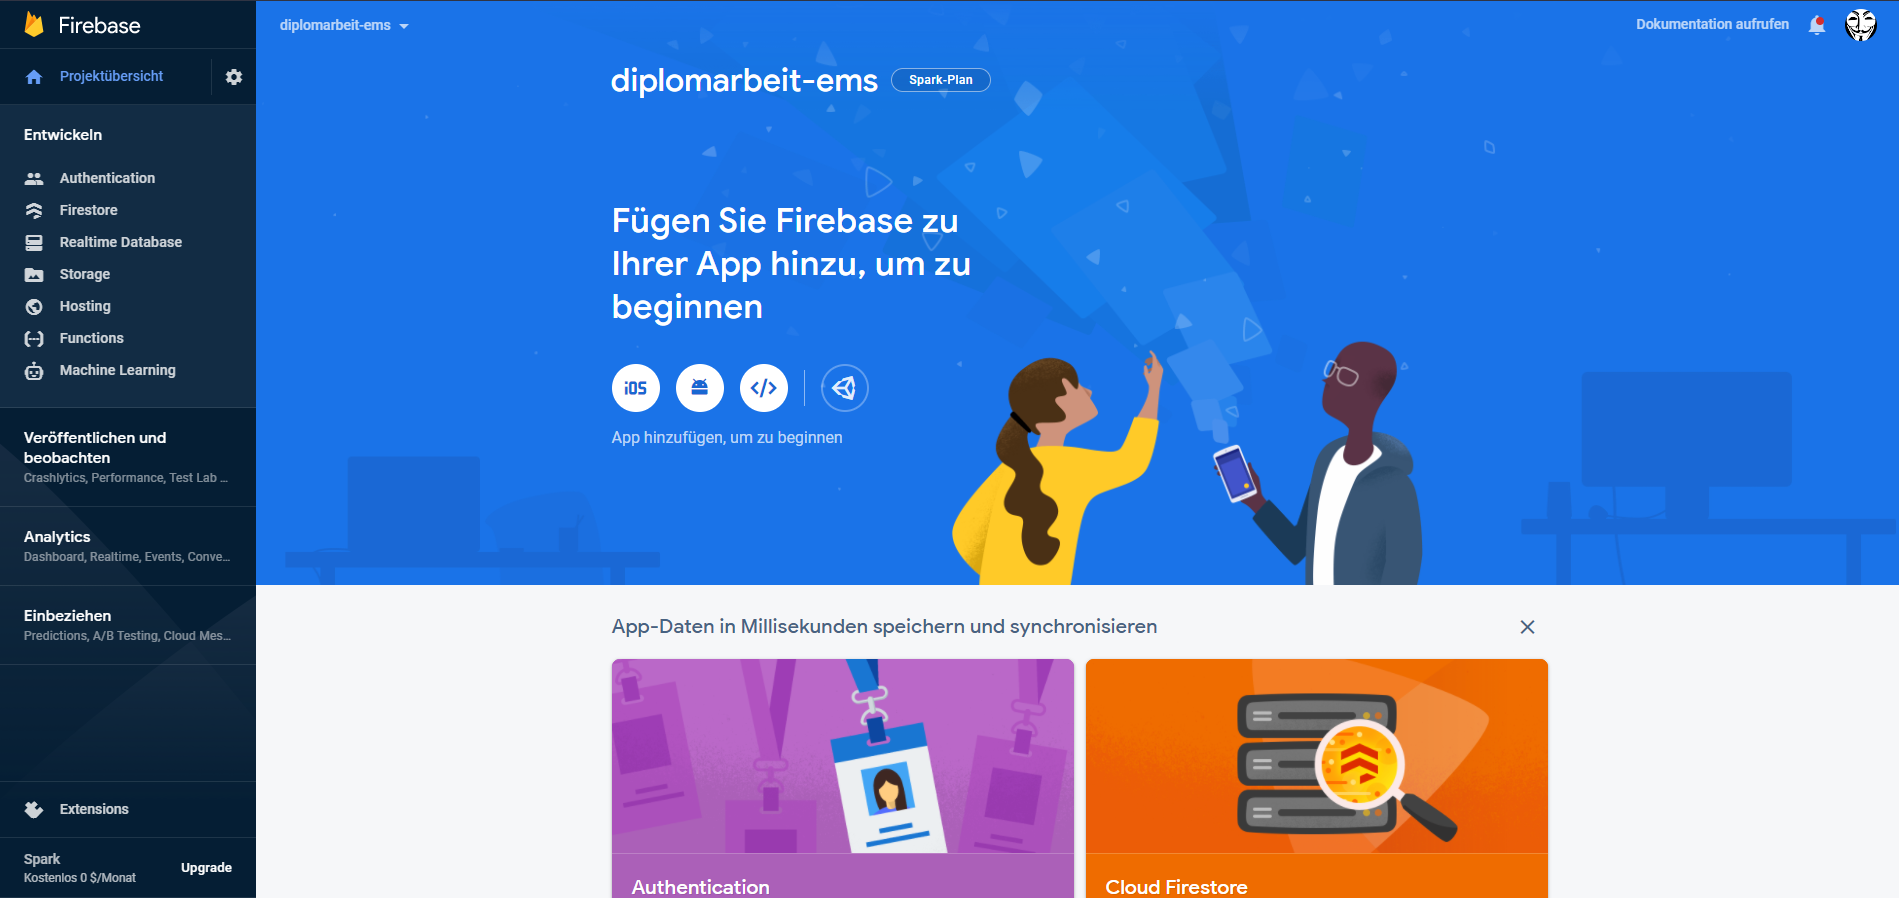
\includegraphics[width=\textwidth]{firebase-main.png}
        \caption{Datenbank erstellen}
    \end{figure}
\end{center}

Nachdem man auf der linken Seite auf "`Realtime Database"' geklickt hat, lädt die Hauptkomponente der Seite neu, nun klickt man auf Datenbank erstellen (Abb. 3.2).

\begin{center}
    \begin{figure}[h]
        \centering
        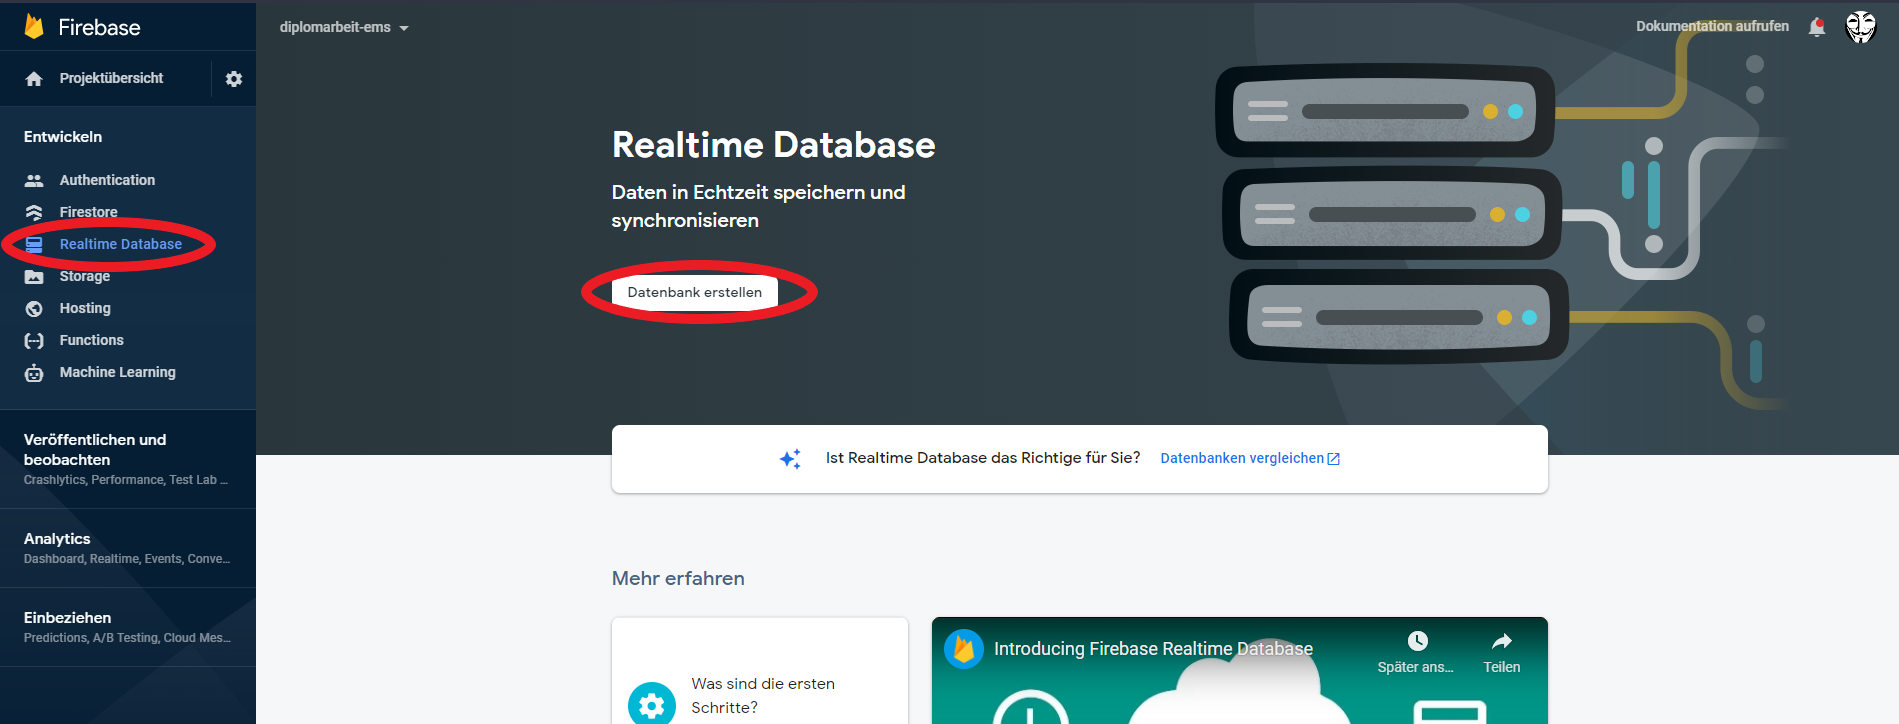
\includegraphics[width=\textwidth]{firebase-db1.png}
        \caption{Datenbank erstellen}
    \end{figure}
\end{center}

Danach erscheint ein Pop-up in welchem man der Ort, wo die Daten der Datenbank gespeichert werden, festgelegt werden. Da die Software DSGVO konform sein muss, sollte ein einen Standort innerhalb der EU aus.

\begin{center}
    \begin{figure}[h]
        \centering
        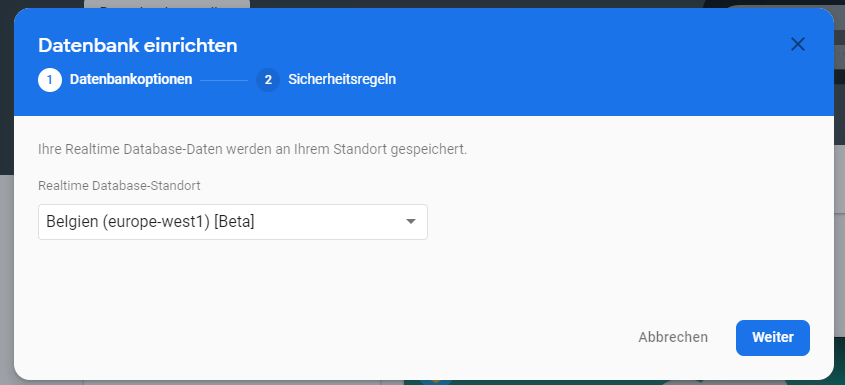
\includegraphics[width=\textwidth]{firebase-db2.png}
        \caption{Datenbank Standort}
    \end{figure}
\end{center}

Mit einem Klick auf Weiter, gelangt man auf die zweite und letzte Seite des Pop-ups. Hier kann man nun auswählen ob die Datenbank direkt in Produktivbetrieb geht oder zuerst der Testmodus gestartet werden soll. Dies ist bei einer
noch aktiven Entwicklung zu empfehlen wie auf den Hinweisen in Abb. 3.3 zu lesen ist.

\begin{center}
    \begin{figure}[h]
        \centering
        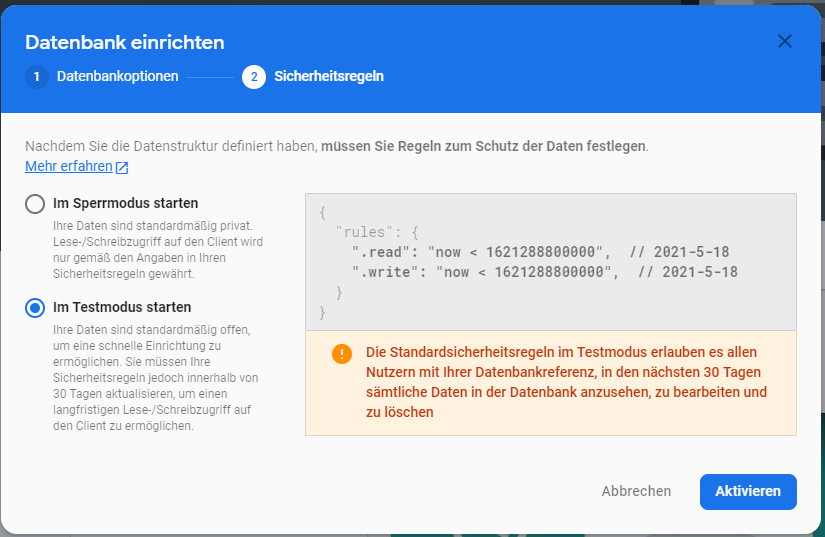
\includegraphics[width=\textwidth]{firebase-db3.png}
        \caption{Datenbank Modus}
    \end{figure}
\end{center}

Nun wurde eine fertige Realtime Database in Firebase erstellt. Damit die nachfolgende Angular App auch mit der Datenbank kommunizieren kann, müssen nur für jetzt zum testen im Testmodus, die Lese- und Schreibrechte auf
jeden übertragen werden. Dies ist in Abb. 3.4 zu sehen.

\begin{center}
    \begin{figure}[h]
        \centering
        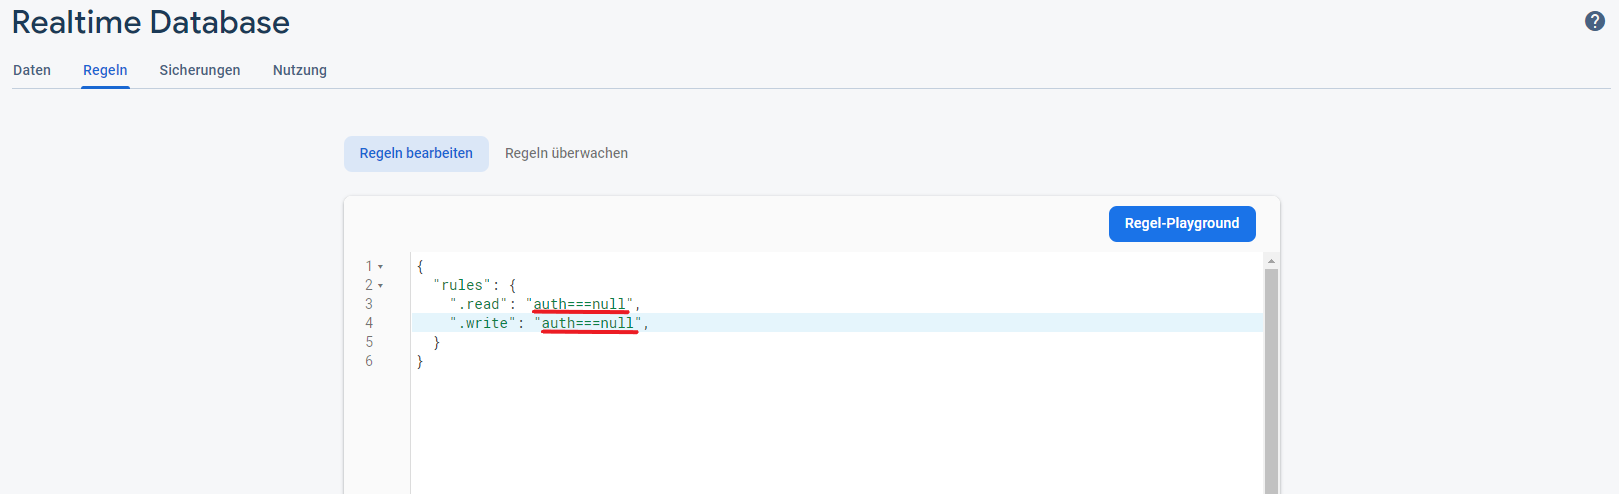
\includegraphics[width=\textwidth]{firebase-db4.png}
        \caption{Datenbank Regeln bearbeiten}
    \end{figure}
\end{center}

Dies war die Konfiguration der Datenbank hinter der Chatapplilation in der Firebase Cloud. Nun folgt eine Anleitung und einige Codesnippets zu Erstellung des eigentlich Chatprogrammes in Angular, welches später in das Hauptprogramm
EMS integriert wird.

Zuerst muss das Google Firebase SDK installiert und auch in einer neuen Angular App inkludiert werden.

\begin{lstlisting}[language=bash]
    #Installieren
    npm install --save firebase

    #In Datei `src/app/app.component.ts` vom Home Verzeichnis 
    #des Projektes aus importieren
    import * as firebase from 'firebase';
\end{lstlisting}

Als nächstes wurden der API Key und die URL zur Datenbank in Firebase gesetzt.



%da war ich https://www.djamware.com/post/5ee1d127711dcf4b441296de/angular-9-tutorial-creating-firebase-chat-web-app#setup-firebase


\newpage

\chapter{Grundlagen der Informationssicherheit}
\strahlhofer

%Reis seine erster Foliensatz
\section{Allgemeines zu Informationssicherheit}
\subsection{Definition}
Bei der Informationssicherheit geht es grundsätzlich darum Informationen zu schützen. Informationen spielen in der heutigen Welt eine wichtige Rolle. Die zwei Arten Informationen zu verarbeiten sind entweder in einer digitalen oder analogen Form. 
\\
Weiters wird überprüft, dass eine fremde, nicht befugte Person oder ein nicht befugtes Unternehmen, auf keinen Fall den Zugriff auf die unternehmensinternen Systeme und Benutzerdaten erhält. Ein Unternehmen muss dafür Maßnahmen setzen, um die Nutzer ihres Services zu schützen. Diese Maßnahmen sollen verschiedenste Bedrohungen vermeiden und zur Datensicherheit, IT-Sicherheit und Datensicherung beitragen.
\\

\section{BSI}

%https://de.wikipedia.org/wiki/ISO/IEC-27000-Reihe
%https://www.onlinesicherheit.gv.at/Themen/Experteninformation/Normen-und-Standards/ISO-IEC-27000.html
\section{ISO/IEC-27000-Reihe}
Die ISO/IEC 27000-Reihe ist eine Ansammlung von Standards über das Informationssicherheitsmanagement (ISMS) und gibt Ratschläge über gewisse Best Practices in diesem Bereich. Sie wurden von der International Organization for Standardization (ISO) und der International Electronic Commission (IEC) publiziert. 
Diese Zertifizierungs-Reihe ist so absichtlich so breit beschrieben, da es für alle möglichen Firmen in jeglicher Größe und Form anwendbar ist.

\subsection{Geschichte}



%https://www.bsi.bund.de/SharedDocs/Downloads/DE/BSI/Grundschutz/Kompendium/Elementare_Gefaehrdungen.pdf?__blob=publicationFile&v=4
%Reis Foliensatz 1
\section{Bedrohungen für Informationssicherheit}
In der Informationssicherheit gibt es viel verschiedene Arten von Bedrohungen die sich laufend verändern. Im BSI sind 47 unterschiedliche Arten von Bedrohungen in der Informationssicherheit aufgelistet.

%bsi und folien von reis
\begin{itemize}
	\item \textbf{Gefährdungen durch natürliche Ereignisse} darunter fallen Naturkatastrophen, Feuer, Wasser, Verschmutzungen durch Staub, Korrosion und ungünstige klimatische Bedingungen die zur Zerstörung der IT-Infrastruktur führen.
	\item \textbf{Ausfälle oder Störungen} diese können von der Stromversorgung, Kommunikationsnetzen, Versorgungsnetzen oder Dienstleistern kommen
	\item \textbf{Schadprogramme} beispielsweise Viren, Würmer, Trojaner, Adware, Spyware, Ransomware
	\item \textbf{Verhinderungen von Diensten (Denial of Service)} auch DoS-Angriffe genannt, versuchen Störungen von Geschäftsprozessen oder IT-Ausfälle herbeizuführen.
	\item \textbf{Social Engineering}, hier gibt sich eine Person als Administrator der eigenen Firma aus. Dieser Angreifer versucht beispielsweise per Telefonat einen Mitarbeiter durch Leichtgläubigkeit dazu  sein Anmeldeinformationen auszugeben.
	\item \textbf{Identitätsdiebstahl} beispielsweise Phishing ist eine Technik die Angreifer verwenden um Kundendaten zu erlangen. Es wird unter anderem eine Anmeldeseite erstellt die identisch zur eigenen ist, um Kunden im Glauben zu lassen, dass sie nichts falsch machen.
	\textbf{Ressourcenmangel} kann auftreten wenn alte Hard- oder Software verwendet wird. 
\end{itemize}

%folien
\section{Gründe für das Informationssicherheitsmanagement}
\paragraph{Gesetzliche Notwendigkeit}
Es liegt eine gesetzliche Notwendigkeit im Sinne des Treffens der geeigneten technischen und organisatorischen Maßnahmen vor, beispielsweise die EU-DSGVO, das Telekommunikationsgesetz, das Urheberrechtsgesetz.

\paragraph{Wettbewerbsvorteil}
Wenn eine Firma einen hohen Stand an Informationssicherheit besitzt, kann sie Konkurrenzfähig bleiben. Zusätzlich kann man mit Partnerunternehmen ins Geschäft kommen, die einen hohen Wert auf Informationssicherheit setzen. Durch Zertifikate kann nachgewiesen werden, dass der Betrieb über ein hohes Sicherheitsniveau verfügt.

\paragraph{Risiken identifizieren}
Ein Vorteil für ein Unternehmen ist das Risiken die mit den Bedrohungen der Informationssicherheit zu tun habe, eher erkannt werden und infolgedessen auch Schäden umgangen werden können.

%https://wotan-monitoring.com/de/news/news-detail/die-schutzziele-der-informationssicherheit-verfuegbarkeit-integritaet-und-vertraulichkeit.html#:~:text=Informationssicherheit%20und%20ISO%2FIEC%2027001&text=Und%20im%20Hauptdokument%2C%20der%20ISO,Vertraulichkeit%E2%80%9C%20und%20deren%20Aufrechterhaltung%20definiert.
%Folien reis
%https://www.bsi.bund.de/SharedDocs/Downloads/DE/BSI/Grundschutz/Kompendium/IT_Grundschutz_Kompendium_Edition2020.pdf%3F__blob%3DpublicationFile%26v%3D6
\section{ISO/IEC 27001}
Die ISO/IEC 27001 definiert sogenannte Schutzziele oder Anforderungen an ein Informationsmanagementsicherheitssystem (ISMS). In dem Dokument wird genau auf die Einhaltung der Bereiche Vertraulichkeit(confidentiality), Integrität(integrity) und Verfügbarkeit(availability) eingegangen. Laut ISO/IEC 27000, gibt es weitere Faktoren die auch ein Teil der Informationssicherheit sein können, das sind Authentizität(authenticity), Zurechenbarkeit(accountability), Nicht-Abstreitbarkeit(non-repudiation) und Verlässlichkeit(reliability).

\subsection{Schutzziele der ISO/IEC 27001}
\paragraph{Vertaulichkeit}
Die Vertraulichkeit beschreibt die Eigenschaft, dass eine Information nicht zugänglich gemacht wird für eine nicht autorisierten Person oder Unternehmen. Somit ist der Schutz gegen Verrat oder Spionage gewährleistet. Darunter wird verstanden, dass Kennzahlen, wie Umsatzzahlen nicht an die Öffentlichkeit gelangen. 


\paragraph{Integrität}
Die Integrität laut dem BSI beschäftigt sich mit der Korrektheit von Informationen. In der Informationssicherheit wird damit assoziiert, dass eine unbefugte Person kein Daten manipulieren kann und darf. Darunter wird verstanden, das Veränderungen wie Datensätze einfügen, verändern oder löschen nicht möglich ist.
Im Rahmen von Integrationstest kann überprüft werden ob Daten von befugten Individuen manipuliert werden, beispielsweise kann dieser Aspekt mittels Hashfunktion überprüft werden.


\paragraph{Verfügbarkeit}
Unter Verfügbarkeit wird in diesem Schutzziel verstanden, dass ein IT-System oder eine Anwendung, für den Benutzer, dass kann ein Mitarbeiter oder ein Kunde sein, jederzeit zu Verfügung steht. Fälle wie, beispielsweise der Ausfall oder nicht Verfügbarkeit durch eine DDoS-Attacke  (Distributed Denial of Service) oder eine DoS-Attacke(Denial of Service) eines Bank-Systems. Wenn das System nicht oder teilweise funktioniert, können möglicherweise keine Überweisungen getätigt werden und folge dessen sind die Angestellten und Konsumenten eingeschränkt. 

%https://en.wikipedia.org/wiki/Man-in-the-middle_attack
\paragraph{Authentizität}
Bei diesem Schutzziel geht es darum, das ein System gewährleistet, dass ein Kommunikationspartner wirklich die Person ist, die er vorgibt zu sein. Bei der Überprüfung der Authentizität muss ein Benutzer sich vorerst authentisieren, dass kann durch viel verschiedene Methoden erfolgen, wie die Eingabe von Benutzername und Passwort oder die Sendung des Reisepasses oder eine Anmeldung via Fingerabdruck oder Gesichtserkennung. Danach kann durch ein Kontrollmodul die Identitätskontrolle an der Person durchgeführt werden und dadurch authentifiziert werden. Am Ende dieses Vorgangs ist eine Person im System angemeldet und es werden im Rahmen der Autorisierung bestimmte Rollen oder Rechte zugewiesen.
Dieses Schutzziel kann Man-in-the-Middle-Angriffe verhindern. Bei dieser Cyberattacke setzt sich eine Person zwischen die Kommunikation zweier verschiedener Parteien und kann damit Transaktionen manipulieren. 

%https://de.wikipedia.org/wiki/Informationssicherheit#Zugangskontrolle
\paragraph{Zugriffssteurung}
Als nächstes Schutzziel gibt es die Zugriffssteuerung. Diese wird gewährleistet wenn der Zugang zu Informationen oder Ressourcen nur autorisiert statt findet, somit wird ein Berechtigungskonzept umgesetzt. Das kann durch verwenden von "individuellen Benutzernamen oder komplexen Passwörtern" erfolgen oder durch eine Authentifizierung durch mehrere Faktoren. In der Praxis werden meist sogenannte Zwei-Faktor Authentifizierungsmethoden verwendet, dass kann beispielsweise durch den Versand eines Codes via Mail erfolgen.

%Reis Folie
\paragraph{Verlässlichkeit}
Bei der Verlässlichkeit geht es darum, dass ein System immer konsistent und nach den festgelegten Spezifikationen läuft. Darüber hinaus soll es zu jederzeit folgerichtige Ergebnisse liefern. Beispielsweise wenn ein System als Hauptfunktionalität das Passwörter verschlüsseln hat, darf es nicht dazu kommen, dass eine inkonsistente Verschlüsselung bei jedem zehnten Benutzer verwendet wird.

%https://en.wikipedia.org/wiki/Information_security#Non-repudiation
\paragraph{Nichtabstreitbarkeit/Verbindlichkeiten}
Dieses Schutzziel gibt an, dass eine Person die ihren Verpflichtungen und Aufgaben aus einem im Vorhinein festgelegten Vertrag nach geht. Des weiteren gilt das wenn ein Beteiligter eine Nachricht erhalten hat, diese nicht abstreiten darf. Infolgedessen darf der andere Beteiligte nicht verleugnen darf die Nachricht versendet zu haben oder eine Datei gelöscht zu haben.


\paragraph{Zurechenbarkeit}
Die Zurechenbarkeit gibt an, dass eine gewisse Aktion oder ein bestimmte Entscheidung einer bestimmten Person die Verantwortlichkeit zugeordnet wird. Dieses Schutzziel ist nicht gegeben, wenn beispielsweise in einem System ein nicht realer Benutzer mit dem Namen "TestUserAdmin" existiert. Wenn dieses Konto für viele verschiedene Personen zugreifbar ist, kann nicht festgestellt werden, wer der Verantwortliche für die Aktionen dieses Accounts ist.


\section{EMS Informationssicherheit}


\newpage
\chapter{Management von Risiken bei Anmeldesystemen}

%Systemplanung und Projekte Entwicklung von Felix Schwab, Ingridschwab-Matkovits
%https://searchcompliance.techtarget.com/definition/risk-management#:~:text=Risk%20management%20is%20the%20process,errors%2C%20accidents%20and%20natural%20disasters.
\section{Risikomanagement im Bereich Anmeldesysteme}
Das Risikomanagement sollte für jedes Unternehmen eine Top-Priorität sein. Durch dieses Verfahren können zukünftige Bedrohungen abgeschätzt und sich dazu Bewältigungsstrategien überlegt werden. Eine Firma muss sich im Vorhinein überlegen welche Risiken eintreten können. Diese Bedrohungen können durch viele verschiedene Ereignisse, wie z.B. durch Naturkatastrophen, rechtliche Verpflichtungen, Managementfehler und sonstige Unfälle eintreten.
Mit der Planung einer neuen oder ausbaubaren IT-Infrastruktur sollte unbedingt das Risikomanagement in Betracht gezogen werden. Die Firma muss versuchen Risiken zu vermeiden oder diese bis zu einem gewissen Grad zu vermindern. 

\begin{center}
\begin{figure}[h]
    \centering
    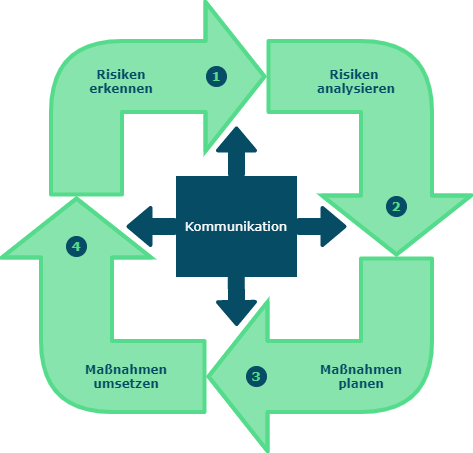
\includegraphics[width=10cm]{Risikomanagement_zyklus.png}
    \caption{Ablauf des Risikomanagements (in Anlehnung auf die Darstellung des BVA)}
\end{figure}
\end{center}

\newpage

\section{Grundbegriffe Risikomanagement}
%Systemplanung und Projekte Entwicklung von Felix Schwab, Ingridschwab-Matkovits
\subsection{Risiko}
Unter dem Begriff Risiko assoziiert man im Bereich IT-Sicherheit die Schadenshöhe, wenn ein bestimmtes Ereignis eintritt. Diese Ereignisse haben einen negativen Effekt auf das Unternehmen. Sie tragen dazu bei, dass materielle oder immaterielle Schäden auftreten können oder sogar Arbeitsprozesse abstoppen.


%Systemplanung und Projekte Entwicklung von Felix Schwab, Ingridschwab-Matkovits
\subsection{Maßnahme}
Eine Maßnahme ist eine Handlung, die ermöglicht ein Risiko zu umgehen oder es einzugrenzen. Hier spricht wird von einer Schadensminimierung gesprochen. 

%https://www.bva.bund.de/DE/Services/Behoerden/Beratung/Beratungszentrum/GrossPM/s-o-s_handbuch/stda_sos-kap8_risikomgmt.html
\section{Ziele des Risikomanagements}
Die Ziele die ein Unternehmen im Blick haben muss sind:
\begin{enumerate}
	\item \textbf{Risiken ausführlich identifizieren:} Die Firma darf keinesfalls essentielle Risiken übersehen.
	\item \textbf{Risiken geeignet bewerten:} Bedrohungen / Risiken sollen in Hinsicht auf die Eintrittswahrscheinlichkeit, mögliche Auswirkungen und auf zeitliche Nähe eingeschätzt werden. Zusätzlich sollen diese darauffolgend mit dieser Betrachtungsweise bewertet werden.
	\item \textbf{Gleichgewicht zwischen Analyse und Umsetzung:} Hier wird versucht eine Balance zwischen Risiken analysieren und dem Auftraggeber und der Projektleitung diese aufzuzeigen zu finden. Zum anderen muss beachtet werden, das Gegenmaßnahmen getroffen werden.
	\item \textbf{Minimierung von Risiken:} Ein Risiko an sich, kann nicht verändert werden. Das Unternehmen kann lediglich durch ein aktives entgegenwirken, die Wahrscheinlichkeit des Eintretens vermindern oder verhindern.
	\item \textbf{Kommunikation:} Dieses Ziel gibt an das die Risiken dem Auftraggeber rechtzeitig übermittelt werden.
	\item \textbf{Überwachung:} Alle diese Ziele müssen für neue oder schon bekannte Risiken immer wieder zyklisch durchgeführt werden. 
\end{enumerate}

\section{Umsetzungsprozesse}
Im Risikomanagement existieren grundsätzlich zwei Arten von Umsetzungsprozessen. Diese unterscheidet man in initiale Prozesse und laufende Prozesse.
Diese beiden Prozesse werden auch als Aufbau Risikomanagement bezeichnet, da alle Vorkehrungen im Vorhinein eines Projekts getätigt werden und als laufendes Risikomanagement, da dieses während der Durchführung des Projekts durchgeführt wird, bezeichnet.

\subsection{Aufbau Risikomanagement}
\subsubsection{Verantwortungszuweisung und Budgetirrung}
Bei der Aufbereitung des Risikomanagements müssen vorher die Rollen jeder einzelnen Personen, die Einfluss auf das Projekt besitzen festgelegt werden. Es wird eine Stakeholderanalyse durchgeführt. Bei dieser Analyse wird herausgefunden welche möglichen Personen, Gruppen oder Organisationen, die in irgendeiner Weise mit dem Vorhaben betroffen sind.
Zusätzlich muss ein Budget festgelegt werden, welches für die Bewältigung eines Risikos eingesetzt wird. Hier muss gegenübergestellt werden wie viel Kosten entstehen falls das Risiko eintritt und wie viel in diesem Fall die Bewältigung kostet.

%https://www.business-wissen.de/hb/risiken-identifizieren/#:~:text=Insofern%20ist%20die%20Identifikation%20von,Sch%C3%A4den%20unvorhergesehen%20und%20%C3%BCberraschend%20eintreten.
\subsubsection{Risikoidentifikation}
Alle Risiken zu identifizieren, die möglicherweise auftreten können, kann sich als sehr schwer erweisen. Es können etwaige Risiken auftreten, von denen noch nichts bekannt war oder die man nicht in Betracht gezogen hat. Aus diesen Gründen spielt die Identifikationsphase eine sehr wichtige Rolle. Sie muss sorgfältig durchgeführt werden und mit verschiedenen Ansätzen abgewickelt werden. Fortlaufend sollte deswegen regelmäßig überprüft werden, ob sich Risiken verändern oder möglicherweise hinzukommen.
\\

%Methoden gefunden: Im Syp Buch
%https://de.wikipedia.org/wiki/Risikoidentifikation#:~:text=Als%20Methoden%20kommen%20f%C3%BCr%20bestehende,oder%20die%20Delphi%2DMethode%20ermitteln.
\subsubsection{Bestehende Risiken und Potenzielle Risiken}
Die Risikoidentifikation beschäftigt sich mit zwei Arten von Risiken auf der einen Hand mit den bekannten Risiken, auf der anderen potenziellen Risiken. Folgende Methoden können zur Bewältigung angewandt werden:
\begin{enumerate}
    \item \textbf{Methoden um bestehende/bekannte Risiken zu identifizieren}
    \begin{itemize}
        \item Einsatz von Checklisten
        \item SWOT-Analyse
        \item Befragungen von erfahrenen Mitarbeitern
        \item Befragungen von Experten mit spezifischen Fachwissen
    \end{itemize}
    \item \textbf{Methoden um Potenzielle Risiken zu identifizieren}
    \begin{itemize}
    	\item Brainstorming
    	\item Brainwriting (bzw. 6-3-5 Methode)
    	\item Delphi-Methode
    	\item Mindmapping
    	\item Morphologischer Kasten
    \end{itemize}
\end{enumerate}

%https://de.wikipedia.org/wiki/Risikoidentifikation#Checklisten_und_Mitarbeiterbefragungen
\subsubsection{Einsatz von Checklisten}
Bei dieser Methode werden standardisierte Checklisten verwendet. Diese sollen einem Unternehmen aufzeigen welche Risiken zu beachten sind, wenn es um die Informationssicherheit geht. Hier besteht jedoch ein Nachteil, denn es werden nicht alle für das eigene Unternehmen relevanten Risiken genannt.

%https://smallbusiness.chron.com/security-swot-analysis-40526.html
\subsubsection{SWOT-Analyse}
SWOT(Strengths, Weaknesses, Opportunities, Threats) ist eine Methode verschiedene Faktoren zu analysieren. 
Durch die Infragestellung stellen der Stärken (Strengths) und der Schwächen (Weaknesses) einer Firma können unternehmensinterne Faktoren identifiziert werden.
Durch hinterfragen von Möglichkeiten (Opportunities) und Bedrohungen (Threats) werden externe Faktoren gefunden, die mit einfließen.


\subsubsection{Stärken}
Eine Stärke von einem Betrieb kann beispielsweise die Verwendung von Firewalls und Anti-Virus Programmen sein. Regelmäßiges Ändern von Passwörtern der Mitarbeiter eines Betriebs kann verhindern, dass eine unternehmens-fremde Person oder andere Unternehmen keinen Zugriff auf die von der Firma genutzten Systeme haben kann.

\subsubsection{Schwächen}
Schwächen müssen erkannt werden und mit Gegenmaßnahmen behoben werden.
Wenn beispielsweise das Unternehmen nicht viel in die Sicherheit eines Systems investiert hat, kann es passieren, dass möglicherweise eine Data Breach(Datenabfluss) auftritt. Die Behebung des Problems wäre, dass alle Firmengeräte einen Virenschutz und einen VPN-Dienst nutzen.

\subsubsection{Möglichkeiten}
In der heutigen Zeit gibt es im Bereich der IT sehr viele verschiedene Anbieter für die unterschiedlichsten Services, wie z.B. Cloud-Services.
Diese Services nehmen dem Unternehmen die Arbeit ab ein eigenes Serversystem aufzubauen und zu verwalten. Dementsprechend wird der Firma geholfen ein Risiko zu vermindern und nimmt dem Betrieb somit einen sehr großen Aufwand ab. 

\subsubsection{Bedrohungen}
In diesem Bereich muss überlegt werden was gemacht werden soll wenn ein Ausnahmefall, beispielsweise eine Naturkatastrophe oder ein Hacking-Angriff, eintritt. Somit muss überlegt werden, wie im Vorhinein gehandelt werden soll. Es muss überlegt werden, wie man die Daten von dem Unternehmen sichert. Das kann durch verschiedene Backup-Strategien sichergestellt werden.


%https://de.wikipedia.org/wiki/Risikoidentifikation#Checklisten_und_Mitarbeiterbefragungen
\subsubsection{Befragungen}
Bei diesen Umfragen werden entweder erfahrene Mitarbeiter oder Experten mit gewissen Fachkompetenzen befragt. Der Vorteil bei der Befragung von Mitarbeitern ist, dass sie eher interne Unternehmensrisiken identifizieren. Bei dem Einsatz von Experten werden eher externe für das Unternehmen bedrohliche Risiken erkannt. Befragungen können in einer digitalen, schriftlichen oder mündlichen Art statt finden.
Wichtig ist es bei diesen Befragungen, dass die Fragen genau zu beschreiben und sie sinnvoll auf das Unternehmen anzupassen.

%Buch S. 38
\subsubsection{Brainstorming}
Hier versammeln sich eine Gruppe von unternehmensinternen Personen bestehend aus bevorzugterweise fünf bis sieben Personen. 
Beim Brainstorming-Prozess werden Vorschläge und Ideen nur verbal geäußert und danach dokumentiert. Eine Person, der sogenannte Moderator leitet diesen Kommunikationsprozess. Vorzugsweise sollte dieser Vorgang nur zehn bis maximal zwanzig Minuten andauern.
Die Bewertung der erhobenen Ideen / Vorschlägen darf nicht gleichzeitig mit der Erhebung ablaufen und darf deswegen nur in einer zweiten Phase abgehalten werden.

Es gibt gewisse Regeln die zu beachten sind:
\begin{itemize}
	\item Keine Barrieren: Das bedeutet, dass eine Person alles vorschlagen kann, auch wenn es eine absurde Idee oder nicht umsetzbar ist. Keine Idee ist zu extrem.
	\item Keine Diskriminierung: Damit ist gemeint, dass kein Teilnehmer für eine geäußerte Idee kritisiert werden soll. Diese Regel ist sehr wichtig, da es sonst den kreativen Prozess stört oder sogar verhindert.
\end{itemize}

%Buch S. 38
\subsubsection{Brainwriting (6-3-5 Methode)}
Bei dieser Methode gibt es sechs Personen die sich zusammensetzen. Jeder Teilnehmer soll dann jeweils 3 Ideen schriftlich festhalten, in einer Zeit von ungefähr 5 Minuten.
Als nächster Schritt wird dann das Schriftstück in der Runde verteilt. Das kann entweder in eine Richtung weiter gegeben werden oder sie werden durchgemischt und dann verteilt. 
Als Ergebnis dieser Methode sollten nach 30 Minuten 108 Ideen aufgeschrieben worden sein.
Der Vorteil dieser Methode ist, dass alle Ideen dokumentiert worden sind und die Ergebnisse deshalb in einer schriftlichen Form vorhanden sind.

%Buch S. 41
\subsubsection{Delphi-Methode}
Bei der Delphi-Methode wird eine Problemstellung oder ein Risiko von einer Gruppe aus verschiedenen und nicht voneinander abhängigen Experten bzw. Fachleuten bearbeitet. 
Jeder Teilnehmer erarbeitet auf einem Schriftstück einen Lösungsansatz, um das gestellte Problem zu lösen.
Die Ausarbeitungen werden eingesammelt und anonymisiert weitergegeben.
Der erhaltene Lösungsansatz soll jetzt kritisiert werden, das heißt falls die Person Denkfehler oder falsche Ansätze verwendet. Aus dieser Bearbeitung soll man für das eigene Konzept Ideen oder Änderungen finden und integrieren.
Dieser Prozess soll mehrere Male wiederholt werden, sodass die Gruppe eine gemeinsame Lösung beschließt.
Die Anonymität spielt bei der Methode eine große Rolle und trägt dazu bei, dass jeder Teilnehmer kreative und alternative Standpunkte einnimmt.
Der Vorteil diese Methode anzuwenden ist, dass unabhängige Fachleute eingesetzt werden und diese über einen größeren Zeitraum an dieser Problematik arbeiten.
Ein daraus folgender Nachteil ist ein hoher Zeit- und Organisationsaufwand.

%https://dieprojektmanager.com/linke-und-rechte-gehirnhaelfte-test/
\subsubsection{Mindmapping}
Das Mindmapping ist eine Methode die angewandt wird um Assoziationen zu einem Thema grafisch darzustellen.
Die Methode ist sehr einfach zu bewältigen und bringt beide Gehirnhälften zum arbeiten. Die linke Gehirnhälfte die analytische Denkprozesse führt und die rechte Hälfte die über den kreativen und intuitiven Teil des Denkens zuständig ist.
\\
%https://de.wikipedia.org/wiki/Assoziation_(Psychologie)
\paragraph{Assoziationen:} 
Eine Assoziationen ist in der Psychologie so definiert, das zu einem Thema gewisse Ideen oder Vorstellungen verknüpft werden. Diese Verknüpfungen können durch eine ausgelöste Emotion oder einen bestimmten Sinneseindruck geschaffen werden. Daraus folgen Denkprozesse zu diesem Thema. 

%Buchseite 40
\paragraph{Durchführung:}
Es wird ein Thema erfasst und z.B. auf ein Whiteboard oder einen Zettel geschrieben. Dies ist das Zentralthema was von der Gruppe behandelt wird.
Darauffolgend werden gewisse Untersektionen erstellt, diese sollen versuchen das Hauptthema aufzuspalten in kleiner Unterthemenpakete.
Die Teilthemen vom Hauptthema nennt man Hauptäste.
Dieses Aufteilungsverfahren kann so oft wie nötig wiederholt werden, in dem die Themen immer weiter aufgeteilt werden, diese werden dann als Zweige bezeichnet.

\paragraph{Regeln:} Bei dieser Methode müssen gewisse Regeln eingehalten werden diese sind:
\begin{itemize}
	\item Das Thema muss in der Mitte des Schreibwerkes liegen.
	\item Das Hauptthema und die Hauptäste des Diagramms sollten in großgeschriebenen Blockbuchstaben festgehalten werden.
	\item Die Linien zwischen Ober- und Unterthema sollten geschwungen sein, da sie dadurch organischer aussehen.
	\item Auf jeder Linie darf nur ein Wort aufgeschrieben sein und die Länge der Linie muss genauso lang sein wie der diesbezügliche Begriff.
	\item Zusätzlich sollen verschiedene Farben oder Symbole für die Themen verwendet werden
\end{itemize}


\subsubsection{Morphologischer Kasten}
Beim morphologischen Kasten werden viele verschiedene Aspekte oder gewisse Merkmale von einer Lösung in eine systematische Reihenfolge angeordnet. Diese Technik soll dazu führen zu erkennen welche ideale Kombination für die Risikobewältigung, verwendet werden kann.

\subsection{Laufendes Risikomanagement}
\subsubsection{Sensibilisierung}
Es muss gegeben sein, dass das Risikomanagement für alle Teammitglieder eine Bedeutung besitzt. So kann sichergestellt werden, dass alle Mitarbeiter sich zu jederzeit bewusst sind, dass Risiken eintreten können. Durch Disziplin und Einhaltung von Protokollen können größtenteils die Mitarbeiter von gewissen Risiken sensibilisiert werden. Geschulte Arbeiter wissen aus diesem Grund, was im Ausnahmefall in den meisten Fällen zu tun ist.

%BVA
%https://de.wikipedia.org/wiki/Risikoanalyse
\subsubsection{Risikoanalyse und Risikobewertung}
Bei diesen beiden Bereichen muss es eine klare Trennung geben. Zuerst sollen eine Risikoanalyse stattfinden und danach eine Risikobewertung, somit kommt es zu einer klareren Übersicht und die Risiken werden genauer bewertet.

%Syp-Buch S.141
\subsubsection{Risikoanalyse}
Bei einer Risikoanalyse sind die Risiken zu betrachten durch die schon durch geführte Risikoidentifikation klar, welche Risiken in einem System eintreten können, die zu Störungen oder Anhalt von Arbeitsprozessen führen. Mit dem Einsatz von einem Ursachen-Wirkungs-Diagramm (auch Fishbone- oder Ishikawa-Diagramm). Dieses Diagramm gibt alle möglichen Ursachen die ein spezielles Ereignis auslösen können an.

%Syp-Buch S.141
\subsubsection{Risikobewertung}
Mittels der Risikobewertung werden von den schon identifizierten Risiken die Eintrittswahrscheinlichkeit eines Ereignisses und die möglichen Folgeschäden bewertet. Die Durchführung einer solchen Bewertung wird mit \textbf{qualitativen} und \textbf{quantitativen Methoden} durchgeführt.

\paragraph{Qualitative Methoden}
Mit qualitativen Methoden wird versucht Risiken anzuordnen nach Höhe der jeweiligen Schadensauswirkung.
Diese Risiken werden nach ihrer "Eintrittswahrscheinlichkeit" und ihren "Einfluss auf den Projekterfolg" eingeordnet. Durch diese Zuteilung in einen gewissen Bereich kann die angemessene Strategie verwendet werden. Die 4-Felder-Methode wird hier verwendet.

\begin{center}
\begin{figure}[h]
    \centering
    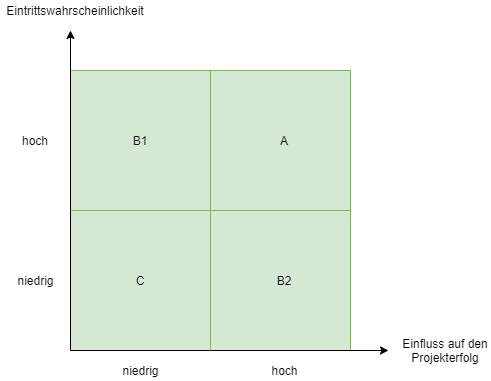
\includegraphics[width=10cm]{4-Felder-Methode.png}
    \caption{4-Felder-Methode (in Anlehnung an die Abbildung im Buch Systemplanung und Projektentwicklung von Felix Schwab und Ingrid Schwab-Matkovits)}
\end{figure}
\end{center}

\begin{itemize}
	\item Bereich A: Hier sind Sofortmaßnahmen durchzuführen, ansonsten könnte es möglicherweise zum Projektende führen.
	\item Bereich B1: Die Risikogestaltung soll mit gewissen Maßnahmen abgewickelt werden.
	\item Bereich B2: Es sollte bei diesem Bereich eine Risikovorsoge mit bestimmten Versicherungen festgelegt werden.
	\item Bereich C: sind Risiken die nicht eine hohe Priorisierung benötigen, diese können am Ende von aller Risiken bearbeitet werden
\end{itemize}

%https://www.risknet.de/wissen/rm-methoden/monte-carlo-simulation/
\paragraph{Quantitative Methoden}
Mit quantitativen Methoden kann man die Schadenshöhe bei Eintritt eines Ereignisses feststellen. Ein Risiko ist wird hier mit einem Geldwert dargestellt.
Das kann durch die Hilfe des Projektstrukturplans festgestellt werden oder mit beschreibenden statistischen Verfahren.

%Bild

\subsubsection{Risikogestaltung}
Bei der Risikogestaltung wird vor Eintritt eines Ereignisses Maßnahmen gesetzt um diese entweder zu verringern oder wenn möglich zu vermeiden.
Es kann bei der Risikogestaltung kann entweder präventiv oder korrektiv vorgegangen werden.

\paragraph{Arten von Maßnahmen zur Risikogestaltung}
\begin{itemize}
	\item Risikovermeidung
	\item Risikoverringerung
	\item Risikoüberwälzung
	\item Risikoübernahme
\end{itemize}

%https://www.computerweekly.com/de/definition/Risikovermeidung
\subsubsection{Risikovermeidung}
Dieser Prozess versucht, dass die Firma einem potenziellen Risiko von Vorhinein gar nicht erst ausgesetzt wird. Das kann durch die Erstellung von Richtlinien, Prozeduren und Schulungen gelöst werden.

%https://strafrecht-online.org/problemfelder/at/tb/obj-zur/risikoverringerung/
\subsubsection{Risikoverringerung}
Bei diesem Prozess werden die internen- als auch externen Risiken betrachtet. es wird versucht diese abzuschwächen oder zeitlich zu verzögern. Durch die Erstellung von gewissen Gegenmaßnahmen kann dann das Risiko verringert werden.

\subsubsection{Risikoüberwälzung}
Hier werden mögliche vertraglich gebundene Verpflichtungen abgeschlossen. Das können z.B. Versicherungen oder Cloud-Services sein. Diese nehmen dem eigenen Unternehmen Risiken ab. Beachtet werden muss das wenn die eigenen Sicherheit verstärkt wird, auch die Kosten dafür steigen. Wichtig zu beachten ist, das solche Abnehmer nur Risiken übernehmen können, worauf dieser Einfluss haben kann.

\subsubsection{Risikoübernahme}
In diesem speziellen Fall geht es um den mögliche Eintritt eines speziellen Risikos. Diese Bedrohung war entweder schon bekannt oder ist vermeintlich unbekannt geblieben. Hier sollten die im Vorhinein geplanten Rücklagen bereit stehen um solche Risiken aufzufangen.

\subsubsection{Regelmäßige Kontrolle}
Die Liste der Gegenmaßnahmen wird genauso, wie die Risikoliste, regelmäßig aktualisiert werden.  


\subsection{EMS Risikomanagement}
Vor Anfang der Erstellung des Anmeldesystems, musste überlegt werden welche Risiken bei der Entwicklung zu beachten sind. Da so ein System viele verschiedene Risiken bergen kann. Aus diesem Grund musste das Risikomanagement durchgeführt werden. Es können dadurch Risiken erkannt, eingeschätzt und bewertet werden. Dementsprechend müssen diese Risiken, durch die Risikogestaltung abgewickelt werden.

\subsubsection{Durchführung des Aufbau Risikomanagements}
\paragraph{Verantwortlichkeit und Budgetirrung}
Am Beginn wurde der Projektleiter(Benjamin Strahlhofer) als der Verantwortliche für dieses Vorhaben festgelegt. Zur Umsetzung und zur Abfederung der Risiken wurde kein Budget festgelegt, da für dieses Vorhaben und für das Gesamtprojekt dies nicht gegeben wurde.


\chapter{Aspekte eines Anmeldesystemes und Biometrie}
\strahlhofer

\section{Prozesse des Anmeldevorgangs}
\begin{center}
\begin{figure}[h]
    \centering
    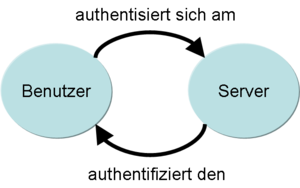
\includegraphics[width=9cm]{authentisieren-authentifizieren.png}
    \caption{Ablauf eines Anmeldevorgangs (Abbildung von wikipedia)}
\end{figure}
\end{center}

%https://www.dr-datenschutz.de/authentisierung-authentifizierung-und-autorisierung/
\subsection{Authentisierung}
Bei der Authentisierung muss von einer Person ein Nachweis gegeben werden, dass sie die Person ist die sie behauptet zu sein. Dieser Nachweis kann durch drei verschiedene Methoden nachgewiesen werden, diese sind:
\begin{itemize}
	\item Die Person besitzt Wissen über eine Information, die nur der Kontoinhaber wissen kann, z.B. das Passwort oder Sicherheitsfragen sein.
	\item Das Individuum das sich versucht anzumelden und sendet beispielsweise einen Reisepass oder Führerschein als Konformation.
	\item Es wird vom Nutzer eine Information mitgesendet die er oder sie nur von sich selbst senden kann. Ein Beispiel wäre die Sendung von einem biometrischen Nachweis, dass kann entweder ein Fingerabdruck oder ein Gesichtsscan sein.
\end{itemize}

%https://www.dr-datenschutz.de/authentisierung-authentifizierung-und-autorisierung/
\subsection{Authentifizierung}
Bei diesem Schritt des Anmeldeablaufs, wird eine Überprüfung durchgeführt. Diese Prüfung soll analysiert die Informationen, die bei der Authentisierung erfasst worden sind. Können diese dem Zielkonto zugewiesen werden, dann ist der Nutzer die Person die er angibt zu sein.

%https://www.dr-datenschutz.de/authentisierung-authentifizierung-und-autorisierung/
\subsection{Autorisierung}
Die Autorisierung hat als Funktionalität die Bestätigung von bestimmten Rechten und Rollen zu bestimmten Ressourcen. Dieses Thema gehört der Informationssicherheit an und befasst sich mit der Zugriffskontrolle. Bei der Autorisierung wird für das Unternehmen ein Zugriffsmechanismus implementiert. Wenn z.B. ein Promoter sich in einem von der Firma erstellten System anmeldet, werden bestimmte Rollen und Rechte zugewiesen. Dies bedeutet das der Mitarbeiter nur einen bestimmten Zugriff auf gewisse Funktionalität besitzt.

\subsubsection{Rollen}
Bei der Anmeldung in die EMS-Software soll zwischen den Rollen Promoter und Administrator unterschieden werden. 
\begin{itemize}
	\item \textbf{Administratoren:} Die Rolle ist eine der wichtigsten in der Software. Dieser kann Benutzer und Events in einem System erstellen, verändern und löschen. Benutzer können zusätzlich deaktiviert werden, da diese entweder zu häufig falsche Anmeldeinformationen eingegeben haben oder weil die Person eine Anfrage darauf gestellt hat.
	\item \textbf{Promoter:} Diese Rolle sind Benutzer der Software, die Karten anfordern und verkaufen können. Sie können, beispielsweise die Funktionalitäten wie die Benutzer- und Eventverwaltung nicht bedienen.
\end{itemize}

%https://www.kaspersky.de/resource-center/definitions/biometrics
%Biometrie
\section{Biometrie}
%https://en.wikipedia.org/wiki/Biometrics
\subsection{Definition}
\begin{center}
	\textit{Biometrics are body measurements and calculations related to human characteristics}
\end{center}

Bei dieser Wissenschaft, schließt eine biometrische Identifikation nur auf eine bestimmte Person.
Durch diesen Aspekt ist die Biometrie eine sehr angesehne Technik in der Identifikation von Menschen.

\subsection{Methoden der Biometrie}
Eine biometrische Information kann durch viele unterschiedliche Methoden erhoben werden.
\begin{itemize}
	%https://www.livescience.com/62690-how-dna-ancestry-23andme-tests-work.html
	%https://www.ibia.org/biometrics-and-identity/biometric-technologies/dna#:~:text=DNA%20Biometrics,often%20in%20forensics%20and%20healthcare.&text=A%20feature%20of%20DNA%20identification,familial%20relationships%20via%20DNA%20testing.
	\item \textbf{DNA-Tests:} Ein DNA-Test wird in den unterschiedlichsten Arbeitsbereichen verwendet, z.B. in der Fornesik oder von der Polizei.
	Vorteile die DNA als biometrisches Mittel zu erwägen:
	\begin{itemize}
		\item Mit der DNA kann von einer unbekannten Person auf dessen Verwandten schließen. Dies ist die einzige biometrische Methode die diese Möglichkeit bietet.
		\item DNA Spuren und Fingerabdrücke können bei Tatorten gefunden werden. Diese Methode hilft Ermittlern schneller die Identität einer Person herauszufinden.
	\end{itemize}
	%https://de.wikipedia.org/wiki/Fingerabdruck
	\item \textbf{Fingerabdruck:} Die Fingerabdrücke sind bei jedem Menschen unterschiedlich. 
	Es gibt bis zum heutigen Tag keine bewissenen Fingerabdruckstest der auf zwei verschiedene Menschen schließen konnte. 
	Nicht einmal eineiige Zwillinge besitzen den gleichen Abdruck.
	Dieser Aspekt macht diese Methode so genau, es wird hier von einer Einzigartigkeit gesprochen.
	\paragraph{Vorteile}
	\begin{itemize}
		\item Wie schon beschrieben werden Fingerabdrücke von Ermittlern verwendet, um die Identität von Opfern oder verdächtigen Personen aufzudecken.
		\item Der Fingerabdruck wird bei den meisten Smartphones in der heutigen Zeit per eingebauten Scanner ermittelt. Diese biometrischen Informationen werden erhoben um das Gerät einer bestimmten Person oder auch Personen zuzuordnen.
	\end{itemize}
	\paragraph{Nachteile}
	\begin{itemize}
		\item In dem Fall, dass scih eine Person auf dem Finger verletzt, kann es dazu führen das der Fingerabdruck sich verändert. Aus diesem Grund kann sich die Person möglicherweise nicht mehr identifizieren.
	\end{itemize}
	%https://en.wikipedia.org/wiki/Facial_recognition_system
	%https://www.pcs.com/wissens-werte/biometrie/gesichtserkennung-von-angesicht-zu-angesicht#:~:text=Hohe%20Sicherheit%20ist%20mit%20Gesichtserkennung,in%20der%20Regel%20nicht%20erkannt.
	\item \textbf{Gesichtserkennung:} Hier wird ein Foto oder Video analysiert und überprüft ob diese Person mit den schon aufgenommenen Bildern in der Dantebank übereinstimmen. Hier werden Aspekte wir Abstand von Augen-Nase-Mund festgestellt.
	\paragraph{Vorteile}
	\begin{itemize}
		\item Eine Person hat keinen oder kaum einen Aufwand um sich bei dieser Methode zu identifizieren. Bei Smartphones muss man lediglich in die Frontal Kamera schauen.
		\item Gesichtserkennungssysteme besitzen den Vorteil mehrere Personen aufeinmal zu erkennen. Beispielsweise in einem Labor dürfen nur bestimmte Personen zutreten. Wenn zwei Personen nun gleichzeitig eintreten wollen und einer die Berechtigung dazu nicht besitzt, wird ein Alarm ausgelöst.
	\end{itemize}
	\paragraph{Nachteile}
	\begin{itemize}
		\item Eineiige Zwillinge können bei dieser Methode schwer unterschieden werden, da diese über ein fast identisches Gesicht besitzen.
	\end{itemize}
\end{itemize}

%https://candytech.in/10-worthy-fingerprint-scanner-smartphones-in-india/#:~:text=Motorola%20was%20the%20first%20company,fingerprint%20scanner%20at%20the%20top.
%https://en.wikipedia.org/wiki/Android_(operating_system)
\subsection{Biometrie auf Android Geräten}
Android ist eine Betriebssystem für Smartphones und Tablets. Der Erfolg des Betriebssystems, zeichnet sich damit aus, dass es Open Source ist. Das bedeutet ein Unternehmen kann Android frei und ohne Kosten nutzen.
\paragraph{Fingerabdruckssensoren}
Motorola hatte im Jahre 2011 das Motorola Atrix veröffentlicht. Dies war das erste Smartphone auf dem Weltmarkt, dass einen Fingerabdruckssensor eingebaut hatte.
Dieses Gerät bekam durch dieses Feature einen sehr hohen Bekanntheitsgrad und löste damit gleichzeitig einen Technologie Trend aus.
Im laufe der danachfolgenden Jahre baute Apple dann auch einen Fingerprintsensor in ihre Geräte ein. Des weiteren begannen dann andere Android Smartphone Hersteller auch diesen Sensor zu integrieren.
Über die Jahre sind viele verschiedene Arten von Sensoren entwicklet worden. Wie z.B.
\begin{itemize}
	\item Berühren eines Knopfes auf dem Gerät (z.B. Apple Geräte).
	\item Wischen über einen Knopf (z.B. Samsung S7 Edge).
	\item In-Display, den Finger auf das Display legen (z.B. Oneplus 8). 
\end{itemize}
\paragraph{Gesichtserkennung}
Die Gesichtserkennung gibt es schon für die meisten Android Geräte. Diese sind häufig sehr unsicher, es exisitieren viel Fälle wo das Feature geknackt worden ist. Aus diesem Grund kennzeichnen die meisten Hersteller diese Methode als unsicher. 
\\
%https://www.kiroku-just-write.de/2020/09/01/gesichtserkennung/#:~:text=Die%20grunds%C3%A4tzliche%20Voraussetzung%20f%C3%BCr%20funktionierende,f%C3%BCr%20jeden%20Menschen%20einzigartig%20sind.
%https://www.consumentenbond.nl/veilig-internetten/gezichtsherkenning-te-hacken
\paragraph{consumentenbond}
Im Jahre 2019 wurde eine Studie von einer niederländischen Organisation zu dem Thema Gesichtserkennung bei Smartphones, durchgeführt. 
Diese haben 60 Smartphones von unterschiedlichen Herstellern getestet. 26 dieser Handys konnten mittels eines Portraits des Telefonbesitzers entsperrt werden.

%https://en.wikipedia.org/wiki/Touch_ID
\subsection{Biometrie auf iOS Geräten}
Apple Inc. ist eine Technologie Firma aus den Vereinigten Staaten, die durch den Verkauf von Computern in den siebziger Jahren. Das Unternehmen bringt jährlich Smartphones(iPhones), Tablets(iPads), Laptops(MacBooks) auf den weltweiten Markt.
\paragraph{Touch ID}
Nachdem 
Im Jahre 2012 kaufte Apple die Firma AuthenTec. Dieses Unternehmen spezialisierte sich auf das Lesen von Fingerabdrücken.
Im darauffolgendem Jahr brachte das Unternehmen dann das iPhone 5s heraus. Dieses Gerät hatte einen Fingerabdruckssensor im "Home-Button" eingebaut. Ab diesem Zeitpunkt konnten alle Benutzer zusätzlich zu ihrem Passwort eine sogenannte Touch ID zur Identifikation benutzen.
Die Fingerabdrücke wurde auf den Chips des Geräts gespeichert, anstatt in der Cloud. Das macht Angreifern es unmöglich die biometirschen Infomrationen abzufangen.
%https://www.pcwelt.de/international/Gesichtserkennung-auf-Android-Smartphones-einrichten-10824319.html
\paragraph{Face ID}
Das erste Smartphone von Apple, dass Gesichstserkennung besitzte, war das iPhone X(2017). Dieses Feature trug den Namen Face ID und löste größtenteils damit die Touch ID ab.
Alle Geräte die Face ID verwenden haben eine 3D-Sensoren die mehr Gesichtsmerkmale erkennen, als wie bei Android Geräten.


\subsection{Biometrie bei EMS}
Bei der Plannung der Software von EMS wurde ein Framework namens Ionic, das auf Angular aufbaut, verwendet. Dieses kann ein Projekt in zwei fast identisch aussehende Applikationen umwandeln, die auf Android und iOS laufen.
In der Dokumentation wurde Fingerprint AIO vorgestellt. Dieses Tool ist eine von Cordova bereitgestelltes Plugin, um einen Fingerabdruck auf iOS und Android zu verwenden.
Dieses Feature kann auch beispielsweise mit Face ID bei iOS Geräten verwendet werden.

\paragraph{Umfrage} Die Gruppe hatte zwei Ideen biometrische Identifikation in die Applikation zu integrieren. Ein Vorschlag war nach dem der Benutzer sich eingeloggt und SSO ausgewählt hat, kann der Fingerabdruck zur Anmeldung verwendet werden.
Eine andere Idee war vor jeder Anfrage die gestellt wurde die biometrischen Daten überprüft werden.
\\
Es wurden dafür 10 verschiedene Personen im Alter von 16 bis 20 Jahren befragt. Das Resultat hatte ergeben, dass 8 von 10 Personen bei jeder Ticketanfrage einen Identifikationsprozess durchführen.
Des weiteren wurde gefragt ob beide Vorschläge realisiert werden sollen. Hier haben 10/10 darauf eingestimmt das nur eines dieser Vorhaben realisiert werden soll. Der Grund war zu meist, dass eine zu häufige Abfrage störrend sein kann.

\paragraph{Umsetzung} Die Biometrie wurde jetzt so umgesetzt, dass vor einer Anfragenstellung der Fingerabdruck überprüft wird.

\section{Passwortzurücksetzung}
Auf fast jeder Website, ist es ein Standard eine Passwortzurücksetzung anfordern zu können. In den meisten Fällen wird diese mittels Link unter der Anmeldung gekennzeichnet, beispielsweise mit der Bezeichnung "Passwort vergessen?".
In diesem Projekt haben wir das Versenden einer Zurücksetzungsmail mit SendGrid. Dies ist ein Anbieter dieser Anbieter macht es möglich leicht E-Mails mittels Node.js zu versenden.
Für das EMS Projekt wurde der kostenlose Tarif gewählt. Dieser kann bis zu 100 Mails an einem Tag automatisiert versenden.

\subsection{Anfrage}
Wenn die Person das Passwort zu ihrem/seinem Account vergessen hat, kann diese durch Eingabe der E-Mail-Adresse eine Passwortzurücksetzungscode erhalten. Wenn auf den Knopf "Senden" gedrückt wird.
Diese Information wird an das Backend weitergegeben und eine E-Mail wird dann mit einem Zurücksetzungscode versandt. 

\begin{center}
\begin{figure}[h]
    \centering
    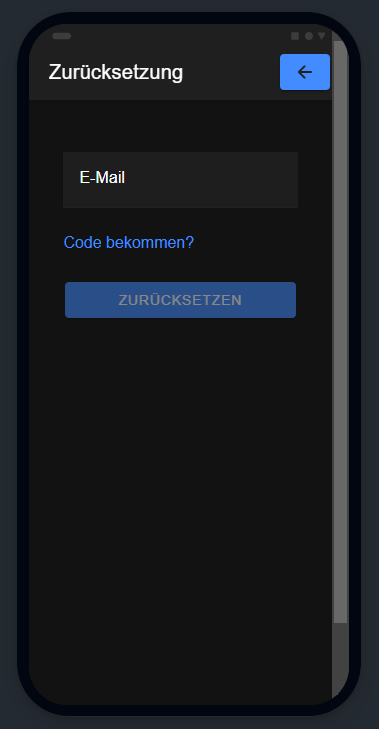
\includegraphics[width=7cm]{pw_anfrage.PNG}
    \caption{Passwortzurücksetzungsanfrage}
\end{figure}
\end{center}
\newpage

\subsection{Zurücksetzung}
Zum Navigieren auf diese Seite muss bei der Anfrageseite "Code erhalten" gedrückt werden. Bei der Zurücksetzung muss die Person vorerst den versendeten Code erfassen. Wenn kein Code erhalten wurde kann man über den Link "Keine E-Mail bekommen" zurück zur Anfrageseite. Als nächstes werden Daten erfasst, wie E-Mail-Adresse, Zurücksetzungscode und zweimal das neue Passwort.
Mittels drücken des "Zurücksetzen" Knopfes wird dann das neue Passwort auf gewisse Faktoren, wie Länge von mindestens 8 Zeichen und Verwendung von einem Großbuchstaben, einem Sonderzeichen und einer Zahl geprüft.
Wenn eine gültige Eingabe getätigt wurde, werden die Daten an das Backend versendet, wo Zurücksetzungscode und E-Mail-Adresse geprüft werden. Wenn ein User mittles diesen Aspekten gefunden wurde, wird das Passwort geändert.

\begin{center}
\begin{figure}[h]
	\centering
	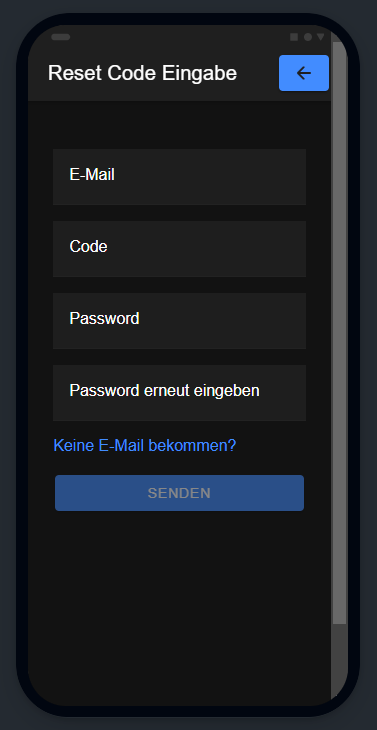
\includegraphics[width=7cm]{pw_eingabe.PNG}
	\caption{Passwortzurücksetzung}
\end{figure}
\end{center}

\chapter{Grundlagen von Datenbanken}
\bauer

	\section{Allgemeines zu Datenbanken}
	
	%Quelle: https://www.oracle.com/de/database/what-is-database/)
	\subsection{Definition}
	Eine Datenbank ist definiert als eine Sammlung von Informationen oder Daten welche im Normalfall auf einem elektronischen Medium wie einer Festplatte abgelegt werden. Der Zugriff auf die Daten erfolgt meist durch ein Verwaltungsprogramm. In den Grundzügen könnte die Daten auch simple Textdateien oder Papier sein welche per Hand befüllt und ausgewertet werden. Dies ist allerdings nicht die Norm. In der Industrie werden meist Datenbankverwaltungssystem benutzt welche von einem externen Anbieter zur Verfügung gestellt werden (Oracle, MongoDatabase, Microsoft SQL Server).
	
	%Quelle: https://www.mongodb.com/nosql-explained/nosql-vs-sql
	\subsection{Arten von Datenbank}
	In der Datenverarbeitung wird grundsätzlich zwischen zwei Arten von Datenbanken unterschieden auf der einen Seite gibt es SQL Datenbank und auf der anderen Seite NoSQL Datenbanken. Einer der größten Unterschiede dieser beiden Datenbank ist wie die Daten strukturiert und abgespeichert werden.
	
	%Quelle: https://de.wikipedia.org/wiki/SQL
	%Quelle: https://www.businessnewsdaily.com/5804-what-is-sql.html#:~:text=%2C%22%20Palic%20said.-,SQL%20history,Data%20Banks%2C%22%20in%201970.
	\subsubsection{SQL (Structured Query Language)}
	In einer SQL Datenbank werden die Daten durch eine klar definierte Struktur in Tabellen gespeichert und auf der Festplatte abgelegt. Die Structured Query Language früher bekannt als "SEQUEL" wurde in den 1970er von Raymond Boyce ond Donald Chaberlin welche damals bei IBM angestellt waren entwickelt. Zu diesem Zeitpunkt war SQL aber noch nicht für die Öffentlichkeit verfügbar, dies kam erst 1979 als eine Firma Namens "Relation Software" welche heutzutage unter dem Namen Oracle bekannt ist ihre Version der SQL Sprache als Oracle V2 auf den Markt gebracht haben.
	
	%Quelle: https://www.mongodb.com/nosql-explained/nosql-vs-sql
	\subsubsection{NoSQL (Not only Structured Query Language)}	
	In einer NoSQL Datenbank können Daten auf verschieden Arten organisiert und abgespeichert werden. Aber sämtliche dieser Methoden Unterscheiden sich vor allem auf eine Art von einer normalen SQL Datenbank. Dieser Unterschied liegt darin, dass die Datenbank nicht in konstanten Tabellen aufgebaut ist und dadurch eine höhere Flexibilität in den Daten ermöglicht. Ein Beispiel für eine solche Flexibilität ist die Speicherlösung welche die Firma "MongoDB" anbietet. In einer NoSQL Datenbank von diesem Anbieter werden die Daten in einzelnen JSON-Dateien geschrieben. Dies ermöglicht das jedes Element wenn benötigt eine eigene Struktur hat ohne das ein Schema vorgegeben oder angepasst werden muss. Eine weitere Sache welche in NoSQL Datenbank möglich ist die in SQL Datenbanken nicht so einfach realisierbar wäre ist die möglich in einem Datenobjekt ein Array von weiteren Datenobjekten zu speichern. Dies ermöglicht eine sehr hohe Flexibilität und war einer der Gründe warum wir uns bei unserem EMS Projekt auch für eine MongoDataBase entschieden haben.
	
	%Quelle: https://www.mongodb.com/nosql-explained/nosql-vs-sql
	\subsection{SQL vs NoSQL}
		Wie bereits vorher Beschrieben gibt es schon im Aufbau und in der Funktionsweise der Datenbank große Unterschiede in diesem Bereich werden die Vorteile und Nachteile der Datenbank Architekturen genauer beschrieben und gegenüber gestellt.
	
	%Quelle: https://becksche.de/Meldung/24-01-2014-sql-oder-nosql
	\subsubsection{SQL Vorteile}
		Um in einer SQL Datenbank etwas zu speichern muss immer ein Schema für die Datenbank vorher entwickelt und implementiert werden. Dieses Schema hat den Vorteil das direkt vom Anfang an bekannt ist welche Daten in der Datenbank gespeichert werden und wie die Datenbank aufgebaut wird. 
		Ein weiterer an dem Tabellen Aufbau ist die Einfachheit der Darstellung da die Daten ähnlich wie in einer Excel Tabelle angezeigt werden. Die Administration in einer SQL Datenbank ist ebenfalls einfacher da ins besondere für die weiter verbreitenden Datenbanksysteme wie Oracle oder Microsoft SQL Server viele Administrationstools existieren.
		
	\subsubsection{SQL Nachteile}
		Einer der Vorteile der SQL Datenbank ist gleichzeitig einer der Nachteile da ein Schema immer entworfen sein muss bevor die Datenbank befüllt werden kann, dies sorgt dafür, dass nachträgliche Änderungen der Struktur schwer zu bewerkstelligen sind da die alten Datensätze entweder aktualisiert oder teilweise mit dem Wert "Null" aufgefüllt werden müssen. Ein weiter Nachteil den viele Entwickler in einer SQL Datenbank sehen ist, dass aufteilen von Informationen über mehrere Tabellen. Wenn eine Datenmodellierung nach dem Lehrbuch durchgeführt wird muss die Datenbank am Ende der Modellierung in der dritten Normalform bestehen was in den meisten Fällen dafür sorgt, dass Daten auf mehreren Tabellen aufgeteilt sind um redundante Daten zu vermeiden. Diese Normalform verkompliziert allerdings oft die Abfragen da Joins benötigt werden um sämtliche Daten zu erhalten. Dazu kommt das diese Abfragen weniger Performant sind da mehrere Tabellen nach Informationen durchsucht werden müssen. 
		
	%Quelle: https://www.mongodb.com/nosql-explained/nosql-vs-sql
	\subsubsection{NoSQL Vorteile}
		Einer der größten Vorteile einer NoSQL Datenbank liegt in der Flexibilität des Datenmodels. Dieses Datenmodel hilft vor allem bei der Entwicklung einer Software wo die Anforderungen an die Datenbank nicht von Anfang an genau bekannt sind. Dies liegt daran, dass nicht von Anfang an ein Schema zum speichern der Daten benötigt wird da die einzelnen Objekte nicht in einer gewöhnlichen Tabelle gespeichert werden. Statt dessen werden die Daten in Objekte gespeichert welche nicht konsistent mit den anderen Objekten sein müssen. Dies bedeutet das es ein Objekt existieren kann welches Attribute besitzt die in den anderen Objekten nicht existieren. Ein weiterer Vorteil einer NoSQL Datenbank liegt darin, dass in einem Objekt ein Array von weiter Objekten gespeichert werden können dies wird in der Fachsprache als verschachteltes Array bezeichnet dies sorgt dafür das eine NoSQL fast nie Beziehungstabellen benötigt was Abfragen oft schneller macht da keine Joins benötigt werden. 
	
	%Quelle: https://www.mongodb.com/nosql-explained/nosql-vs-sql
	%Quelle: https://www.dnsstuff.com/de/nosql-datenbankvergleich#:~:text=Nachteile%20von%20NoSQL%2DDatenbanken&text=Erstens%20bieten%20NoSQL%2DDatenbanken%20nicht,wodurch%20ihre%20Systeme%20komplexer%20werden.
	\subsubsection{NoSQL Nachteile}
		Einer der Nachteile einer NoSQL Datenbank liegt darin das diese Datenbanken meist das ACID-Prinzip (Atomarität, Konsistenz, Isolation , Dauerhaftigkeit) nicht einhaltet was in manchen Fällen zu einer inkonsistent führen könnte. Allerdings gibt es die Möglichkeiten das die Entwickler ihren eigenen Code implementieren welcher das ACID-Prinzip einhält dies führt aber oft zu einem komplexeren Datenbanksystem. Ein weitere Nachteil der NoSQL Datenbank besteht darin, dass diese nicht mit der SQL-Sprache kompatible sind was die Lernkurve vor allem bei Entwicklern welche bis jetzt SQL verwendet haben erheblich anheben kann. Dazu kommt das Abfragen insbesondere wenn diese komplexer werden manchmal Performanceeinbußen entstehen können.
		

	\subsection{Datenbankentwurf}
		Der Datenbankentwurf umfasst alle alle Aufgaben zur Ermittlung der Struktur einer Datenbank. Das Entwerfen dieses Modell wird in 4 Phasen Unterteilt.
		
		\subsubsection*{Zweckbestimmung}

		\subsubsection*{Konzeptionelles Modell}

		\subsubsection*{Logisches Modell}

		\subsubsection*{Physisches Modell}


	\subsection{EMS Datenbank}
		In diesem Bereich wird auf den Datenbankaufbau in unseren Diplomarbeitsprojekt genauer eingegangen und die Gründe für unsere Entscheidungen sowohl den Aufbau betreffend als auch den Anbieter.
		
		%Quellen: https://www.mongodb.com/company#:~:text=MongoDB%20was%20founded%20in%202007,the%20shortcomings%20of%20existing%20databases.
		\subsubsection{Technologie}
			Für die EMS-Software hat sich unser Team für die MongoDB entschieden. Diese Datenbank baut auf JSON ähnliche Objekte auf welche Dokumente genannt werden. Jedes Dokumenten repräsentiert einen Datensatz, mehrere Dokumente sind in einer Kollektion zusammengefasst. Jedes Dokumenten hat beim erstellen einen Identifikator welche bei MongoDB mit '\_id' abgekürzt wird. Dieser Identifikator ist in der gesamten Datenbanken eindeutig, dass ist möglich da es sich um eine hexadezimal 12-Byte Zahl handelt. 
		
		\subsection{Anbieter}
			Unser Team hat sich für den Anbieter Atlas entschieden welcher Großkunden wie Adobe und Google. Die Firma wurde im Jahr 2007 von Dwight Merriman, Eliot Horowitz und Keyvin Ryan gegründet welche auch die Entwickler der Firma DoubleClick sind. Bei diesem Anbieter kann sich jeder eine gratis Datenbank erstellen welche über eine geteilte Cloud zur verfügbar gestellt wird. Für Geld kann die Datenbank auch direkt über Atlas auf einem dediziertem Server aufgesetzt werden welche zwischen 5€ und 1000€ pro Tag kosten können. Theoretisch könnte MongoDB auch auf seinem eigenen Rechner laufen lassen allerdings hat sich unser Team dagegen entschieden da die Administration von 4 nicht zentralen Datenbank während der Entwicklung ein zu großer Aufwand gewesen wäre
		
		\newpage		
		\subsubsection{Aufbau}
			Die Datenbank selbst ist in 2 Kollektionen aufgeteilt die Kollektion 'events' und die Kollektion 'users'. In der Kollektion 'events' werden alle Informationen zu einem spezifischen Event gespeichert und in der Kollektion 'users' werden die individuelle User der Applikation gespeichert sowohl Administratoren so wie die Promoter. Im nächsten Abschnitt werden die einzelnen Datenfelder der Dokumente benannt und der Verwendungszweck beschrieben.

			\subsubsection{Event Aufbau}			
				\begin{itemize}
					\item 'name' der Name des Events wird vor allem für die Anzeige benutzt
					\item 'creation\_date' das Datum gespeichert zudem ein Event erstellt wurde wird hauptsächlich in der Statistik verwendet
					\item 'expire\_date' das Datum gespeichert ab welchen Zeitpunkt es nicht mehr möglich ist Kartenverkäufe über die Applikation einzutragen wird benutzt um den User darin zu hindern Karten zu verkaufen nachdem die Zeit abgelaufen ist
					\item 'description' eine kurze Beschreibung des Events gespeichert um vor allem dem User die Identifikation einfacher zu machen
					\item 'early\_bird\_phase' eine Flagge gesetzt um zu speichern ob bei diesem Event eine Vorverkaufszeit aktiv
					\item 'early\_bird\_close' das Datum gespeichert wann einer der Administratoren die Vorverkaufszeit geschlossen hat
					\item 'cards' besteht aus einem Array aus Objekten
					\begin{itemize}
						\item card\_id' wird benutzt um Karten zu identifizieren (10 stellige zufällig generierte Nummer). 
						\item 'name' der Name der Karte
						\item "early\_bird" ist eine Flagge welche anzeigt das diese Karte nur als verkauft eingetragen werden kann während die Flagge 'early\_bird\_phase' aktiv ist
						\item 'amount' beschreibt die Anzahl an Karten die dieses Event hat
						\item 'price' ist der Preis der spezifischen Karte
					\end{itemize}
					\item 'packages' besteht aus einem Array aus Objekten
					\begin{itemize}
						\item 'package\_id' ist wie 'card\_id' ein Identifikator für die Packages (10 stellige zufällige Nummer)
						\item 'price' der Preis der spezifischen Karte
						\item 'name' der Name des Pakets
						\item 'price' der Preis des Pakets
						\item 'people' die Anzahl an Personen für die dieses Paket geplant wurde
						\item 'description' speichert die Details des Pakets
					\end{itemize}
					\item 'goodies' besteht aus einem Array aus Objekten
					\begin{itemize}
						\item 'goodie\_id' ist wie 'card\_id' und 'package\_id' ein Identifikator für die Belohnungen (10 stellige zufällige Nummer)
						\item 'name' der Name der Belohnungen
						\item 'points' die Punkte die benötigt werden um die Belohnung einzulösen
						\item 'description' die genauere Beschreibung der Belohnungen
					\end{itemize}				
				\end{itemize}
			
			\begin{figure}[h]
				\centering
				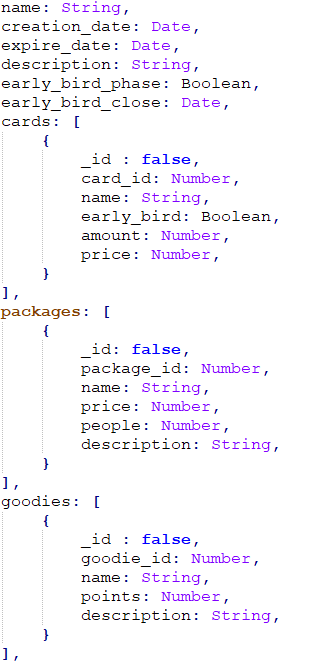
\includegraphics[width=\textwidth,height=\textwidth,keepaspectratio]{events_models.png}
				\caption{Event-Model}
			\end{figure}	
			
			\newpage		
				
			\subsubsection{User}
				\begin{itemize}
					\item 'firstname' der Vorname des User wird vor allem für die Anzeige benutzt
					\item 'lastname' der Nachname des User wird vor allem für die Anzeige benutzt
					\item 'username' der Username des User wird für das ein einloggen verwendet
					\item 'password' das Passwort des Users welches verschlüsselt abgespeichert wird
					\item 'email' die Email Adresse eines User wird vor allem zum Passwort zurücksetzen verwendet
					\item 'active' eine Flagge welche angibt ob ein User momentan aktiv seinen Kartenstand verändern kann
					\item 'admin' eine Flagge welche angibt ob dieser User ein Administrator ist
					\item 'description' eine kurze Beschreibung der Person die jeder User selbst verändern kann
					\item 'resetkey' der Schlüssel mit dem das Passwort zurückgesetzt wird wird nur für interne Überprüfungen benutzt
					\item 'request' eine Flagge welche angibt ob ein User eine Passwortzurücksetzung angefordert hat wird ebenfalls nur für interne Überprüfungen verwendet
					\item 'events' besteht aus einem Array von Objekten indem alle Events des Users gespeichert werden
					\begin{itemize}
						\item 'event\_id' ist die Identifikation des Events um welches es sich in diesem Objekt handelt (ObjektId des Events) in einer SQL Architektur würde man dies den Fremdschlüssel nennen
						\item 'active' eine Flagge welche angibt ob dieser User momentan bei diesem Event seinen Kartenstand verändern darf
						\item 'promotion\_start' das Datum an dem dieser User das Event das erste mal zugeteilt wurde wird für die Statistik verwendet
						\item 'points' der momentane Punktestand des User
						\item 'last\_changed' das Datum an dem der User das letzte mal seinen Kartenstand zu diesem Event aktualisiert hat
						\item 'mone\_submitted' der Betrag den der User bisher von den verkaufen Karten und Paket abgegeben hat
						\item 'cards' ist ein weiteres Array von Objekten
						\begin{itemize}
							\item 'card\_id' die Identifikationsnummer dieses Kartentyp
							\item 'amount' die Menge an Karten die ein User von diesem Kartentyp insgesamt bekommen hat
							\item 'sold' die Anzahl an Karten die der User von diesem Kartentyp verkauft hat
							\item 'submitted' die Anzahl an Karten die der User von diesem Kartentyp zurückgegeben hat
							\item 'available' die Anzahl an Karten von diesem Kartentyp welche der User noch im besitzt hat
						\end{itemize}
						\item 'goodies' ist ein weiteres Array von Objekten indem die eingelösten Goodies gespeichert werden
						\begin{itemize}
							\item 'goodie\_id' die Identifikationsnummer dieses Belohnungstyp
							\item 'date\_of\_redeem' das Datum an welchem diese Belohnung das letzte mal verändert wurde
							\item 'amount' Anzahl an Einlösung für diese Belohnung
						\end{itemize}
					\end{itemize}
				\end{itemize}

			\begin{figure}[h]
				\centering
				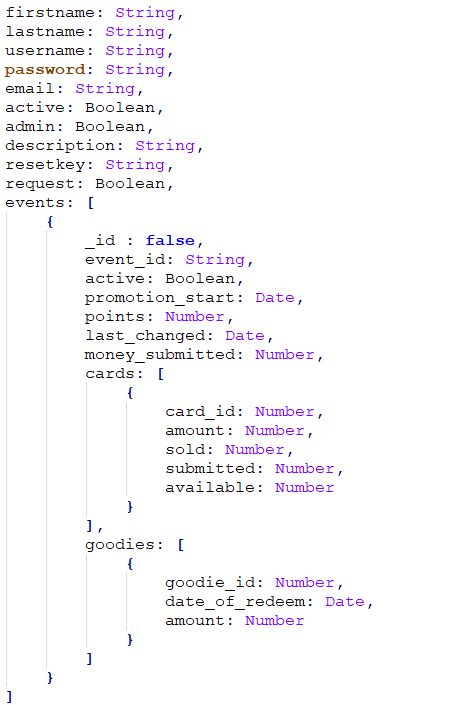
\includegraphics[width=\textwidth,height=\textwidth,keepaspectratio]{user_model.png}
				\caption{User-Model}
			\end{figure}
		
		\newpage
		\subsubsection{Entscheidungsgrundlagen}
			Einer der Gründe warum wir uns für die MongoDB entscheiden haben war, dass am Anfang niemand vorhersagen konnte wie genau unsere Datenbank aufgebaut sein wird. Während der Entwicklung gab es viele Informationen welche nachträglich in die Struktur eingefügt wurden dies hat uns dieser Anbieter sehr vereinfacht. Ein weiter Grund war, die Möglichkeit ein Array aus Objekten zu speichern was viel Abfragen und logistische Probleme gelöst hat ins besondere da wir in unserem Backend über die Schnittstelle "mongoose" auf die Datenbank zugreifen welche einiges ermöglicht was mit MonogDB alleine nicht realisierbar wäre wie zum Beispiel das Vorgeben einer Struktur welche aber veränderbar ist und auch ohne Update auf veralte Datensätze immer noch funktioniert. Diese Struktur ist hat uns auch ermöglicht das alle Mitglieder des Teams einen Überblick über die Datenbank bekommen und einfach Abfragen, Updates und Inserts schreiben konnten. Dazu kommt, dass durch die Möglichkeit der Arrays aus Objekten nur 2 Tabellen (Kollektion) benötigt werden während in einer normalen SQL Datenbank welche in dritter Normalform ist mindestens 12 Tabellen benötigt werden. Natürlich war uns die Performanz der Abfragen sehr wichtig was ein weiter Grund war warum wir uns für diese Technologie entschieden haben da die MongoDB eine sehr hohe Performanz hat selbst beim Abfragen von großen Dokumenten wie sie in unsere Datenbank gespeichert sind. Da die Objekte der MongoDB wie JSON Objekte aufgebaut sind hat das die Auswertung am Backend ebenfalls erleichtert.

\newpage
\chapter{Grundlagen von Data Analytics}
\bauer
	
	\section{Data Analytics}
	
		%Quellen: https://en.wikipedia.org/wiki/Data_analysis
		\subsection{Definition}
			Data Analytics ist ein Prozess bei dem Daten inspiziert, gereinigt, verwandelt und modelliert werden um neue nützliche Informationen zu bekommen. Dies Dient vor allem als Hilfestellung bei wichtigen Entscheidungen. Eines der Ziele von Data Analytics ist es Firmen dabei zu unterstützen effizienter zu arbeiten. 
	
		\subsection{Vorgehensweise}
		
			\subsubsection{Anforderungen}
				Zuerst muss festgelegt werden welche Daten analysiert werden, woher diese Daten kommen und wie die Daten aufgebaut sind. Dies hängt meistens von dem Zweck der Datenanalyse ab. Ein weiter Punkt welcher beachtet werden muss ist das Ergebnis welches erwartet wird von der Analyse.
			
			\subsubsection{Sammlung}
				Die Sammlung der Daten kann von verschiedenen Quellen stattfinden sowohl firmenintern als auch externe Quellen wie das Internet oder externe Datenbanken. Bevor mit der Analyse begonnen werden kann müssen die Quellen erkannt und strukturiert werden. Die Datenmenge muss in diesem Schritt ebenfalls in Betracht gezogen werden. Wenn sich um eine geringe Datenmenge haltet kann die Analyse meist auf einem der Server statt finden welche normalerweise für andere Prozesse verwendet werden. Eventuell reicht bei sehr kleinen Datenmengen auch der Standrechner von den Personen welche die Analyse durchführen. Bei sehr großen Mengen kann es passieren, dass für den Prozess ein extra Server gekauft oder gemietet werden muss. 
			
			\subsubsection{Verarbeitung}
				Bei der Verarbeitung werden die verschiedenen Datenquellen in eine Struktur gebracht welche alle für die spätere Verwendung benötigt wird diese unterscheidet sich je nach Anwendungsfall. Bei diesem Prozess muss darauf geachtet werden das keine der wichtigen Informationen verloren gehen. 
			
			\subsubsection{Reinigung}
				Während der Reinigung werden redundante so wie nicht benötigte Informationen gelöscht dies reduziert die Datenmengen was für besser Performance und einen geringeren Speicherverbrauch sorgt. Dies ist besonders bei großen Datenmengen sehr wichtig. Bei der Reinigung können in vielen Fällen Muster oder auffällige Daten erkannt werden, welche oft einen Ausblick auf das zu erwartenden Ergebnis liefert. 
			
			\subsubsection{Erkundung}
				Durch die Erkundung werden bisher unbekannte Zusammenhänge in den unterschiedlichen Quellen erkannt. Dies kann durch verschiedene Verfahren erreicht werden. Eines der meist verwendeten Methoden ist die explorative Datenanalyse welche ein Teilgebiet der Statistik ist. Dieses Verfahren wird meistens von Diagrammen wie Box-Plot oder Mosaik-Plot unterstützt weiterhin gibt es verschiedene Softwares wie GeoDa oder MANET welches oft kostenlos sind. 
				 
			\subsubsection{Modellierung}
				In der Modellierung werden verschiedene Algorithmen auf die Daten angewendet dies dient vor allem dem Entdecken von Zusammenhänge welche durch die explorative Datenanalyse nicht erkannt werden konnte. 
			
			\subsubsection{Kommunikation}
				Während der Kommunikationsphase werden die Ergebnisse in verschiedenen Formen präsentiert meist unterstützt durch graphische Diagramme welches die effiziente Kommunikation unterstützen. Bei dieser Präsentation sollte daran gedacht werden, dass viele der Entscheidungsträger für welche die Information gedacht ist sich oft nicht mit technischen Spezifikationen aufhalten möchten. 
			
		% Quelle: https://hackr.io/blog/what-is-data-analysis-methods-techniques-tools
		\subsection{Analyse Methoden}
		
			\subsubsection{Qualitative Analyse}
				In der Qualitative Analyse werden die Fragen "wie?" "was?" und "warum?" indem quantitative Techniken angewendet werden  wie Fragebögen oder Einstellungsskalierungen. Diese Analyse kommt für gewöhnlich in Form von Text was eventuell auch durch Audio und Video unterstützt wird. 
				
			\subsubsection{Quantitative Analyse}
				Diese Form der Analyse ist mit Zahlen gestützt die Daten werden an klar definierten Werten festgelegt welches die Darstellung durch Graphen ermöglicht. 
				
			\subsubsection{Text Analyse}
				In dieser Art der Analyse wird Text analysiert um Fakten zu extrahieren welche von Maschinen verstanden werden können. Das Ziel darin liegt strukturierte Information aus unstrukturierten Inhalten zu erstellen. Diese Form der Analyse wird auch als "Text-Mining" bezeichnet.
			
			\subsubsection{Statistische Analyse}
				Bei der statistischen Analyse werden Datensammlungen, Interpretation und Validierungen verwendet um verschiedene statistische Operationen durchzuführen. Die meisten Daten die verwendet werden sind beschreibende Daten wie Fragebögen oder Beobachtungsdaten. 
			
			\subsubsection{Diagnostische Analyse}
				Die diagnostische Analyse ist eine Weiterführung der statistischen Analyse welche eine genauere Analyse ermöglicht. Diese Art der Analyse wird auch als Ursachenanalyse bezeichnet. Die Funktionsweise dieser Art von Analyse kann in drei Kategorien eingeteilt werden. \newline
				Anomalien identifizieren: In dieser Kategorie werden bestimmte Bereiche identifiziert welche genauere Analysen benötigen. \newline
				Bohr Analyse: In dieser Kategorien werden Datenquellen identifizierte dies hilft besonders beim erklären von Anomalien. Diese Form der Analyse benötigt oft Strukturen welche außerhalb der Daten liegen was bedeutet das externe Daten zur Analyse hinzugefügt werden müssen um alle Zusammenhänge zu erkennen.  \newline
				Klausel Zusammenhänge: In dieser Kategorien werden bisher unbekannte Zusammenhänge erkannt durch Wahrscheinlichkeitstheorie, Regressionsanalyse, Filterung und Zeitreihendatenanalyse wodurch versteckte Sachverhalte erkannt werden.  		
			
			\subsubsection{Vorausschauende Analyse}
				In der vorausschauende Analyse werden historische Daten in einen künstliche Intelligenz eingespielt um kritische Muster und Trends zu erkennen. Dieses Model wird danach auf die aktuellen Daten angewendet um zukünftige Trends zu erkennen. 
	
		\subsection{EMS Statistik}
			Die EMS-Software verwendet Data Analytik insbesondere in dem Interface der Administratoren da dieser einen Überblick über die gesamten Aktivitäten der User und über die Events benötigen.  

\chapter{Grundlagen der Rest API}
\bauer
%Quelle: https://en.wikipedia.org/wiki/Representational_state_transfer
\section{Definition} 
REST\footcite{rest} steht für 'Representational State Transfer' und wird oft zum Erstellen von interaktiven Applikationen insbesondere in der Webentwicklung verwendet. Wenn die Applikation dem Prinzip,der Rest Software Architektur folgt, so nennt man diese auch Restful. Die Architektur selbst beschreibt den Zugriff und die Veränderung von Ressource mit einem Zustandslosen Protokoll. Eine Rest API ist somit eine Anwendungsschnittstelle auf die durch ein zustandsloses Protokoll zugegriffen wird.			
%Quelle: 
\section{Geschichte}
Roy Fielding schrieb im Jahre 2000 seine Dissertation über den REST-Architekturstil, allerdings findet die korrekte Umsetzung erst seit dem 2014 Anklang in World Wide Web.		 	
%Quelle: https://restfulapi.net/
\section{Prinzipien}		 				 	
\subsection{Zustandslosigkeit}
Jede Anfrage auf dem Server muss sämtliche notwendige Informationen zur Ausführung der Anfrage enthalten, was bedeutet das sämtliche Session Daten nur auf dem Client gespeichert werden müssen.		 	
\subsection{Caching}
Jede Antwort der Schnittstelle muss als "cachable" oder "non-cacheable" gekennzeichnet sein, damit der Client alle Informationen für die er nicht eine erneute Anfrage an den Server schicken muss, abspeichern kann. Dies erspart sowohl dem Client, als auch dem Server selbst Rechenzeit.		 	
\subsection{Einheitliche Schnittstellen}
Da der Client getrennt vom Server agieren kann und nur Anfragen an diesen schickt, ist es möglich mit einer Rest API eine Schnittstelle für mehrere Geräte zu entwickeln, da zum Beispiel eine Smartphone App die gleiche Schnittstelle wie eine Website verwenden könnte.		 	
\subsection{Mehrschichtige Systeme}
Das System soll aus mehreren Ebenen aufgebaut werden, allerdings sieht der Client selbst nur eine Schnittstelle, was das Interagieren vereinfacht. Der große Vorteil liegt darin, dass dieses System die Abkapslung durch eine Firewall so wie eine einfache Skalierbarkeit bietet.		 	
%Quelle: https://de.wikipedia.org/wiki/Node.js
\section{Node.js}
Node.js\footcite{nodejs} ist eine open-source Javascript Laufzeitumgebung, welche plattformübergreifend arbeitet. 
Die Laufzeitumgebung wird oft dazu verwendet, um Webbrowser aufzusetzen. 
Dieser läuft dann über die JavaScript-Implementierung V8, ursprünglich wurde die Technologie für Google Chrome entwickelt. 
Das Besondere an der Architektur ist, dass sie sehr ressourcensparend ist und dabei eine sehr große Anzahl von Netzwerkverbindungen gleichzeitig zulässt. 
Da bei der Entwicklung von Node.js ein besonderer Fokus auf Performance gerichtet wurde, kommt in dieser Architektur die nonblocking I/O zum Einsatz anstatt der üblichen blocking I/O. Dies sorgt dafür, dass ein Prozess weiterarbeiten kann, obwohl er noch auf Ergebnisse wartet.
Wie zum Beispiel von einer Berechnung oder einer Datenbankabfrage. 		 	
%Quelle: https://en.wikipedia.org/wiki/Node.js#:~:text=Node.js%20was%20written%20initially,and%20later%20sponsored%20by%20Joyent.
%Quelle: https://hostingtribunal.com/blog/node-js-stats/#gref
\subsection{Geschichte}
Node.js wurde ursprünglich von Ryan Dahl in 2009 entwickelt. 
Im Jänner 2010 kam der nächste große Schritt für Node.js, da zu diesem Zeitpunkt der Package Manager (npm) erschien, welcher Programmierer auf der ganzen Welt eine einfache Methode gab Quellcode in Form von so genannten Packages zu entwickel und zu verbreiten. 
Im Juli 2011 kam die erste Node.js Version für Windows, da die früheren Versionen nur unter Linux und Mac OS X veröffentlicht wurden. Im Jahr 2018 hatte Node.js die 1 Milliarde Downloads. Heutzutage wird Node.js für über 20 Millionen Webseiten verwendet. 		 		
%Quellen: https://www.yuhiro.de/vorteile-und-nachteile-von-node-js/
\subsection{Vorteile}
Ein großer Vorteil der Node.js Laufzeitumgebung ist die Performanz welche geboten wird. 
Diese Performanz fällt besonders bei einer großen Anzahl von Verbindungen, beziehungsweise Anfragen auf. 
Dazu kommt die Kompatibilität von Node.js sowohl zu verschiedenen Datenbanken als auch mit fast allen Frontendapplikationen, da das ganze nach Rest-Prinzip aufgebaut ist. 
Natürlich dürfen auch die Packages nicht außer acht gelassen werden, da es über 600.000 davon gibt und jeden Tag neue hinzugefügt werden.		 		
%Quellen: https://www.yuhiro.de/vorteile-und-nachteile-von-node-js/
\subsection{Nachteile}
Bei Updates von Node.js kann es passieren, dass Codes angepasst werden müssen, da es zu fehlenden Rückwärtskompatibilitäten kommen könnte. 
Dies liegt allerdings nicht direkt an Node.js, sondern an dem Javascript Framework an sich. Ein weiter Nachteil ist, dass diese Laufzeitumgebung eine relativ neue Technologie im Vergleich zu PHP oder ASP.NET ist, welche schon viele Jahre mehr verwendet werden. 		 		
%Quellen: https://de.wikipedia.org/wiki/JSON_Web_Token
%Quellen: https://en.wikipedia.org/wiki/Express.js#:~:text=js%2C%20or%20simply%20Express%2C%20is,standard%20server%20framework%20for%20Node.
\section{EMS Rest API} 
Unser Team entschied sich ebenfalls für ein Node.js Backend, um genauer zu sein haben wir uns für Express.js entschieden, welches ein Backend-Webframework für Node.js ist. 
Abgesehen von Express verwendet der Server Mongoose um eine Verbindung mit der Datenbank aufzubauen und den JSON Web Token\footcite{web-token} kurz JWT, welcher es uns ermöglicht nach RFC 7519 genormte Access-Token zu generieren und zu überprüfen. 		 	
\subsection{Express.js}
Express.js oder auch Express genant, erschien am 16.11.2010 und wurde von TJ Holowaychuk programiert, welcher Express als Server mit minimalen Funktionsweisen, aber einer großen Menge von Erweiterungen beschreibt. 
Der große Unterschied zwischen Express und Node.js liegt darin, dass Express ein Framework basierend auf Node.js is, welches vor allem auf Web-Applikationen ausgelegt ist und einige Prinzipien und Methoden von Node.js für diesen Zweck verändert oder sogar Funktionen hinzufügt. 
Dies macht das entwickeln von Web-Applikation mit Express einfacher. 	
%Quellen: https://www.accentsconagua.com/articles/code/an-introduction-to-mongoose-for-mongodb-and-node-js.html
\subsection{Mongoose}
Mongoose ist ein Javascript-Framework welches Zugriff auf die MongoDB vereinfacht. 
Mongoose bietet eine Menge an Funktionen zum Erstellen und zum Arbeiten mit Schemen. 
Ein Schema ist eine abstrakte Beschreibung zu den Dokumenten in einer MongoDB. Auch Abfragen, Updates und löschen wird durch Mongoose vereinfacht, besonders wenn es sich um Dokumente handelt welche Arrays aus Objekten enthalten. 		 	
\newpage
\subsection{Funktionen}
In diesem Teil werden einige der wichtigsten Funktionen beschrieben, welche von unserem Team implementiert wurden und wofür diese benötigt werden. 		 	
\subsubsection{'add\_event\_to\_user'}
Diese Post Funktion wird aufgerufen, wenn einem User ein neues Event zugewiesen wird. 
In dieser Funktion wird ein temporäres Event Objekt erstellt, welche alle notwendigen Daten von der Request speichert. 
Dieses Objekt wird in einem Array gespeichert, welches bei einem spezifischen User in der Datenbank festgehalten wird. 
Falls beim Speichern ein Fehler auftritt, wird der Datenbankfehler an das Frontend geschickt, anderen Falls wird der geänderte User zurück gesendet. 
Diese Funktion ist die Grundlage für die EMS Software, da ein User ohne Events weder Karten bekommen kann noch seinen Kartenstand eintragen kann.		 		
\begin{figure}[H]
	\centering
	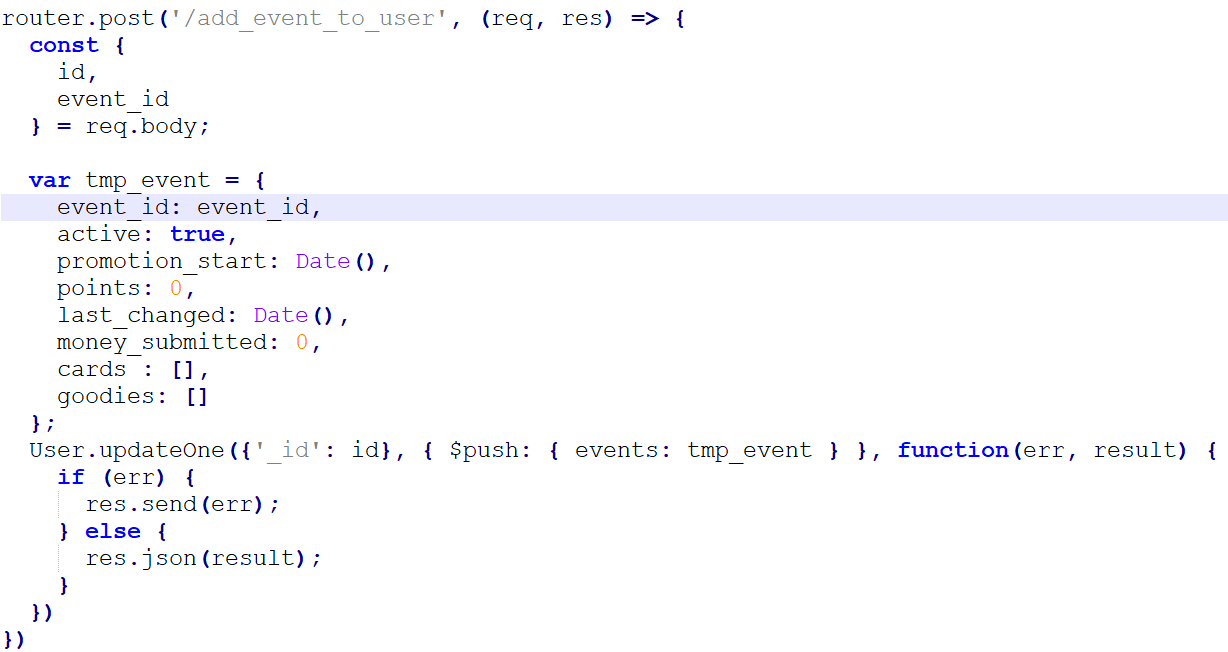
\includegraphics[width=\textwidth]{add_event_to_user.png}
	\caption{'add\_event\_to\_user' Funktion}
\end{figure}	 	
\newpage
\subsubsection{'create\_user'}
Diese Funktion ist ebenfalls eine Post Funktion welche verwendet wird, um einen neuen Promoter oder Administrator in der Datenbank anzulegen. 
Die meisten Daten werden aus der Request gespeichert, allerdings werden drei der benötigten Datenfelder vom Server ausgefüllt und das Passwort wir durch eine externe Bibliothek gehascht. 
Danach wir ein temporäres Objekt erstellt, welches alle für das Erstellen benötigte Daten umfasst. 
Dieses Objekt wird über Mongoose in die User Kollektion gespeichert. Diese Funktion bildet einen Teil der Grundlage, da die EMS Software für eine große Anzahl von Usern ausgelegt ist. 		 		
\begin{figure}[H]
	\centering
	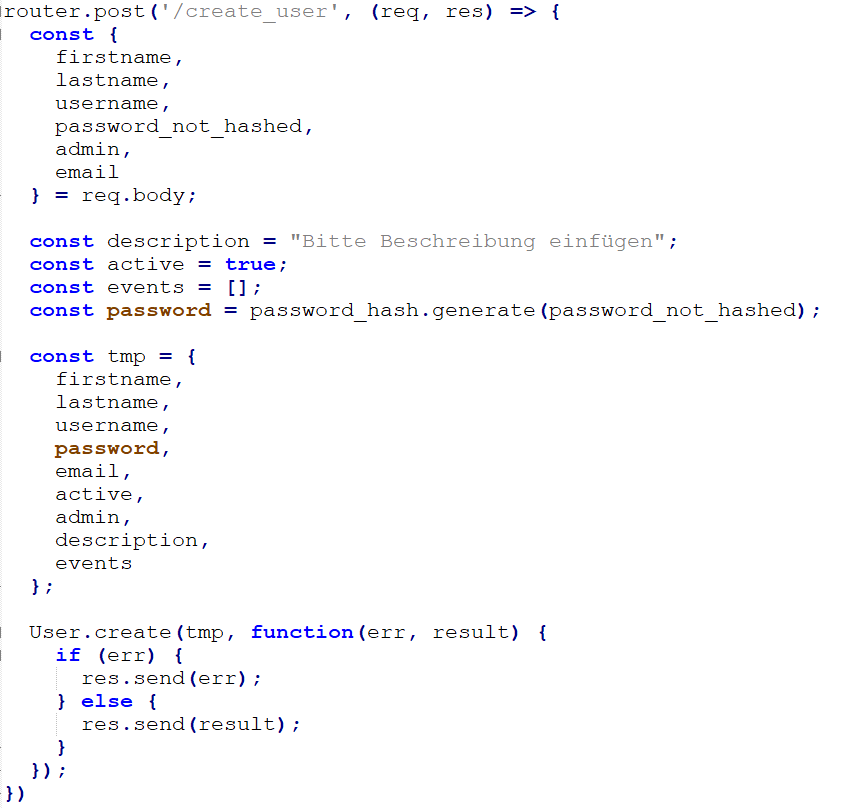
\includegraphics[width=\textwidth]{create_user.png}
	\caption{'create\_user' Funktion}
\end{figure}		 	
\newpage	
\subsubsection{'authenticateToken'}
'authenticateToken' ist eine Middleware welche vor dem ausführen sämtlicher Funktion überprüft, ob im Kopf der Anfrage ein gültiger JWS-Token mitgeschickt wurde. 
Falls ein ungültiger oder falscher Token mitgeschickt wurde, wird der Vorgang abgebrochen und eine Fehlermeldung an das Frontend gesendet. 
Wird ein gültiger Token mitgeschickt, wird die Anfrage nach der Überprüfung wie gewollt ausgeführt. 
Diese Zwischensoftware hilft mit der Sicherheit der Website, da keine Anfragen direkt an den Server geschickt werden können ohne das sie von einem eingeloggten User oder Administrator stammen. 		 		
\begin{figure}[H]
	\centering
	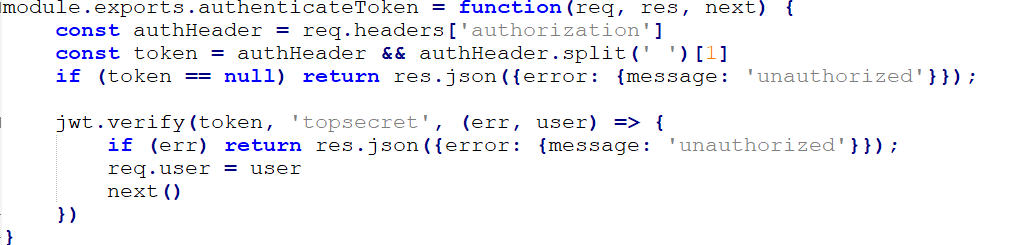
\includegraphics[width=\textwidth]{authentication_middleware.png}
	\caption{'authentication' Middleware}
\end{figure}

\chapter{Ticketsysteme}
\reiter

  \section{Ticketsysteme}
  
  %Quellen: https://www.smartsheet.com/how-use-smartsheet-it-ticketing-system https://de.wikipedia.org/wiki/Issue-Tracking-System 
  \subsection{Anmerkung}
  Da dieses Dokument eine Event-Management-Software behandelt, in der Tickets, also Eintrittskarten verwaltet und an Promoter vergeben werden, besteht die Gefahr, dass diese Ticketverwaltung mit einem Ticketsystem, also einem Issue-Tracking-System, verwechselt werden kann.  
  
  \subsection{Definition}
    Ein Ticketsystem, auch Issue-Tracking-System oder Service-Tracking-System, hat die Aufgabe, alle eingehenden Anfrage von internen und externen Stellen zu verwalten. IT-Abteilungen haben ein sehr hohes Volumen von Meldungen, die bewältigt werden müssen. Somit wird ein System benötigt, dass jede einzelne Meldung während des gesamten Lebenszyklus von Eingang bis hin zur Lösung verwaltet. \\
Es werden verschiedene Dienste bereitgestellt die von einfacher Intake-Software bis hin zu anspruchsvollen Tools, mit denen Probleme ermittelt und verfolgt werden können, reichen. \\
Ticketsysteme sollen IT-Teams über den Status von Tickets, also gemeldete und formell festgehaltene Probleme, auf dem Laufenden halten und Ihnen helfen, Problemlösungen für diese zu entwickeln. 
Ein Ticket enthält in der Grundform ein technisches Problem, eine Beschreibung des Problems und gegebenenfalls Informationen, die es ermöglichen, dieses Problem zu replizieren. \\
Ticketsysteme ermöglichen es der IT-Abteilung effizienter zu funktionieren, indem alle Informationen über Probleme, für die die IT-Abteilung Verantwortung trägt, so schnell wie möglich zu lösen, in einem zentralen Datenspeicher in ausreichender Form beschrieben gespeichert werden. \\
Erfolgreiches Issue-Tracking kann einem Unternehmen helfen Entwicklungskosten von Software zu verringern, da Probleme die frühzeitig behandelt werden einfacher zu beheben sind als jene, die durch fehlende Infrastruktur eines Tracking-Systems erst später behandelt werden können. \\
  
  \subsection{Funktionsumfang eines Ticketsystems}
  
  \begin{itemize}
	  \item 	\textbf{Self-Service-Portal}: Soll einen One-Stop-Shop darstellen, in dem Kunden und Mitarbeiter ihre Tickets schnell und einfach an die zuständige Abteilung des Unternehmens schicken können. Self-Service-Portale vereinfachen den Kontakt zwischen Kunden bzw. Mitarbeiter und der zuständigen Stelle, indem es genau eine Kontaktstelle gibt. Somit können unnötige Anrufe und E-Mail-Verkehre vermieden werden und optimieren somit den Workflow.  \\
	  \item \textbf{	Organisationssystem:} Nach Eingang eines Tickets in das System ist der erste Schritt, dieses zu protokollieren. In der Regel werden den Tickets eine prägnante Kategorie, eine Dringlichkeit, eine geschätzte Zeit bis zur Lösung, Fristen und eine Beschreibung, um das Problem, dass das Ticket beschreiben soll, reproduzierbar zu machen, zugewiesen. Die Tickets werden dann in ein Organisationssystem gespeichert und für die Abarbeitung zur Verfügung gestellt.  \\
	  \item \textbf{Zuweisen von Tickets:} Um den Workflow des Support-teams zu optimieren, sollten Tickets im Prinzip des One-Stop-Shops, einen „Eigentümer“, also einen Mitarbeiter, der sich ausschließlich um dieses Ticket kümmert, zugewiesen bekommen.
	  \item \textbf{	Sicheres System:} Ticketsysteme sollten sicher sein und somit muss eine hohe Priorität auf die Sicherheit im Auswahlverfahren einer Implementierung gesetzt werden. Informationen, die in einem Ticketsystem gespeichert werden, können interne, systemkritische Probleme beschreiben und müssen damit mit höchster Vertraulichkeit behandelt werden. \\
	  \item \textbf{Live Support:} Ein rund um die Uhr besetzter Helpdesk mit Live-Chat Funktionalität vereinfacht die Meldung von Problemen und fördert somit die Bereitschaft von Kunden und Mitarbeitern aufgetretene Fehler in der Software zu melden und in Kooperation mit dem Support-team in einer ausreichenden Form zu beschreiben. Der Helpdesk kann bei technischen Problemen, die keine Softwareänderung vermögen, oder auf Seiten des Kunden oder Mitarbeiters entstanden sind mit bereits bekannten Workarounds helfen. Ebenfalls können redundante Tickets vermieden werden, indem das Support-team kein neues Ticket schreibt, dessen Problem schon erfasst und formell festgehalten wurde. \\
  \end{itemize}
  
  Die nachstehenden Funktionen können den Support-Betrieb weiter optimieren
  
  \begin{itemize}
			\item \textbf{Unterstützung für mehrere Kanäle:} Es kann ebenfalls sinnvoll sein, andere Kanäle, wie Telefon, Videochat oder E-Mail, zum Informationsaustausch zur Verfügung zu stellen. Komplexe Probleme können leichter gelöst werden, wenn man in direktem Kontakt mit dem Support-Personal steht. Fragen zu zusätzlichen Themen können beantwortet und Probleme leichter geschildert und mit Hilfe des Personals festgehalten werden. Es bleibt dennoch nur ein formaler Prozess zur Erfassung von Problemen und Formalisierung in ein Ticket bestehen. \\
			\item \textbf{Dateianhänge:} Kann zur besseren Verständlichkeit des Tickets beitragen. Besonders bei Problemen technischer Natur kann es Hilfreich sein, wenn Informationen wie Memorydumps oder Log-Dateien für den Support zur Verfügung gestellt werden können. Kann zur besseren Verständlichkeit und der Reproduktion von Fehlern eingesetzt werden. Wenn Dateianhänge zugelassen werden sollen, muss ein Dokumentenverwaltungssystem implementiert werden.\\
			\item \textbf{Mehrsprachige Systeme:} Betrifft hauptsächlich internationale Systeme. Ein Mehrsprachiges Support-System kann dennoch universell sinnvoll sein, da Konversationen in der Muttersprache des Kunden für diesen angenehmer und leichter zu verstehen sind und somit die Bearbeitungszeit der Support-Abteilung verringern können. Internationale Systeme können verschiedensprachige Support-teams einstellen, die die gewonnen Informationen in einer einheitlichen Sprache, meistens Englisch, im Ticketsystem festhalten. Unternehmen, mit kleineren Budgets können Echtzeitübersetzungsdienste implementieren. \\
			\item \textbf{Anpassung:} Es ist Sinnvoll, Ticketsysteme mit Orientierung an Plug-and-Play-Prinzipien zu entwickeln, da somit der Funktionsumfang des Systems an die Anforderungen des Projekts angepasst werden kann und eine spätere Erweiterung des Ticketsystems vereinfacht wird. \\
		\end{itemize}  
Die genannten Funktionen stellen allein nicht zwingend sicher, dass das Ticketsystem so effektiv wie möglich funktioniert. Es ist wichtig Kunden, Mitarbeitern und Supportern einen Weg einzurichten, Feedback oder Beschwerden zu äußern und auf dieses zu hören und sich aktiv an der Verbesserung und Anpassung des Ticketsystems zu halten. \\
Eine Implementierung eines Berichtssystems, in dem wichtige Metriken und Analysen wie die durchschnittliche Zeit bis zur Problemlösung, Einhaltung von Fristen usw. festgehalten werden kann ebenfalls die Qualität und Effizienz des Supports steigern. \\
Community-Foren und regelmäßige Feedback-Umfragen können beim Aufbau und der Pflege von Beziehungen zwischen Support und Kunden helfen und ein Gefühl von Rechenschaftspflicht und Vertrauen erzeugen.
%Quelle(n): https://www.datanyze.com/market-share/project-management--217/jira-market-share 
\subsection{Marktanalyse}  
Die zunehmenden Anforderungen an Softwareprojekte erzeugen eine steigende Notwendigkeit, fehlerfreie Projekte erfolgreich durchzuführen und die immer weiter steigenden Investitionen in die IT-Branche beschleunigen das Wachstum des weltweiten Issue-Tracking-Markts. \\\\
Die mögliche Erhöhung des Return-Of-Investments eines Entwicklers, dass durch die Senkung der Entwicklungskosten bei frühzeitiger Erkennung, Behandlung und Behebung eines Bugs entstehen kann, steigert ebenso die Nachfrage und somit die Wachstumsrate des Markts. \\\\
In der folgenden Grafik werden die Marktanteile von den meistverwendeten Ticketsystemen zur Schau gestellt. \\
Jira sticht hier mit 37.86 Prozent Marktanteil als eindeutiger Marktführer heraus. Microsoft Project hat mit 19.09 Prozent einen im Vergleich zu den Nachfolgern einen immer noch sehr hohen Marktanteil.
\begin{figure}[H]
 	\centering
    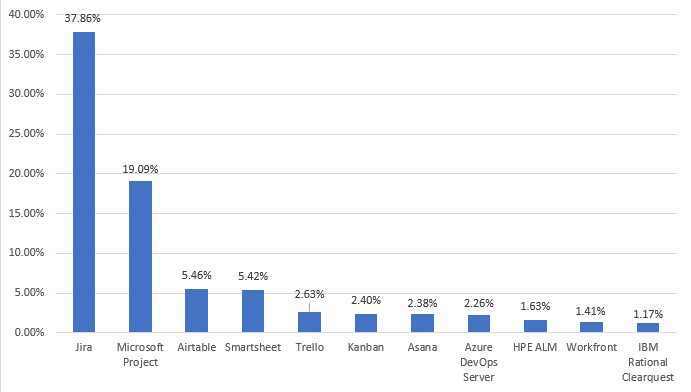
\includegraphics[width=\textwidth]{Marktverteilung_Ticketsysteme.png}
	\caption{Ticketsystem-Marktverteilung}
\end{figure}   
\subsection{Vergleich von Ticketsystemen verschiedener Anbieter}
Es werden die Merkmale der Programme mit Issue-Tracking-Funktionalität
		\begin{itemize}
			\item Jira
			\item Microsoft Project
			\item Airtable
			\item Smartsheet
			\item Trello
		\end{itemize}
gegenübergestellt.   

		\subsection{Vergleich}
		
			%Quellen: https://www.atlassian.com/de/software/jira/features/bug-tracking 
			% https://www.atlassian.com/de/software/jira/pricing 
			Jira
			
			Jira ist ein proprietäres Issue-Tracking-Programm, dass es den Benutzern auch ermöglicht, agiles Projektmanagement zu führen. Jira bietet eine Umfangreiche Implementierung an, die es ermöglicht, Bugs vom Backlog bis zur Behebung zu verfolgen, es können Nachrichten über den aktuellen Status des Fehlers versendet werden, Fehlern können Prioritäten zugewiesen werden, usw… \\
			
			 Eckdaten:
				\begin{itemize}
					\item Kosten: 0\$/Monat Free, 7\$/Benutzer/Monat Standard, 14\$/Benutzer/Monat Premium, Enterprises auf Anfrage
					\item Erstveröffentlichung: 2002
					\item Marktanteil: 37.86\%
				\end{itemize}
				
				Merkmale:
				\begin{itemize}
					\item Native Issue-Tracking-Software
					\item Mächtige Implementation des Ticketsystems
				\end{itemize}
				

				
				%Quellen: https://www.microsoft.com/de-at/microsoft-365/project/compare-microsoft-project-management-software
				%https://support.microsoft.com/en-us/office/add-an-issue-to-a-project-in-project-online-3e1a59e5-43b3-4281-9cfb-503c646f49b9 
				
				Microsoft Project
				
				Microsoft Project ist eine Projektmanagementsoftware, die über eine sehr leichte Implementierung eines Ticketsystems verfügt. Man kann lediglich Issues in einem Project erstellen und wieder löschen.
				
				Eckdaten:
				\begin{itemize}
					\item Kosten: 8.40€/Monat Project Plan 1, 25.30€/Monat Project Plan 3, 46.40€/Monat Project Plan 5
					\item Erstveröffentlichung: 1984
					\item Marktanteil: 19.09\%
				\end{itemize}
				
				Merkmale:
				\begin{itemize}
					\item Schwache Implementierung des Ticketsystems
				\end{itemize}
				

				
				%Quellen: https://support.airtable.com/hc/en-us/articles/115003131627-Use-case-bug-issue-tracking-in-Airtable 
				%https://airtable.com/templates/product-design-and-ux/expOzMycWirMsUOTL/bug-and-issue-tracker 
				%https://airtable.com/pricing 

				Airtable
				
Airtable ist ein Cloud-basierter Kollaborationsdienst der mittels vom Entwickler bereitgestellten Bug Tracker Templates eine Funktionserweiterung als Issue-Tracking-System erhält. Issues können auf einem Kanban board oder auf einem Grid angezeigt werden. Screenshots und Gifs können dem Ticket hinzugefügt werden. Verfügt über mächtige Filteroptionen.

				
					Eckdaten:
				\begin{itemize}
					\item Kosten: Free, 10\$/Monat Plus, 20\$/Monat Pro, Auf Anfrage Enterprise Package
					\item Erstveröffentlichung: 2012 
					\item Marktanteil: 5.46\%
				\end{itemize}
				
				Merkmale:
				\begin{itemize}
					\item Screenshot- und Gif-attachment der Tickets
					\item Mächtige Filteroptionen
					\item Cloud-basiert
				\end{itemize}
				

				
				%Quellen: https://www.smartsheet.com/how-use-smartsheet-it-ticketing-system
				% https://de.smartsheet.com/pricing 
				
				Smartsheet
				
				Smartsheet ist eine über Software-as-a-Service laufende Projektmanagement Software und hat ein eingebautes Ticketsystem namens Help Desk Ticket Tracker \& Form. Es optimiert die Ticketverwaltung, indem es interne und externe Tickets organisiert und stellt einen Helpdesk zur Verfügung. 
				
					Eckdaten:
				\begin{itemize}
					\item Kosten: 13€/Monat Einzelbenutzer, 22€/Monat Business, Enterprise auf Anfrage
					\item Erstveröffentlichung: 2006
					\item Marktanteil: 5.42\%
				\end{itemize}
				
				Merkmale:
				\begin{itemize}
					\item Software-as-a-Service
					\item Native Implementation eines Ticketsystems.
					\item Stellt einen Helpdesk zur Verfügung.
				\end{itemize}
				
				
				%Quellen: https://blog.trello.com/how-to-transform-trello-into-a-powerful-bug-tracker-with-the-marker-power-up
				% https://trello.com/de/pricing 
				
				Trello
				
				Trello ist ein Aufgaben-Verwaltungs-Onlinedienst der mittels Marker-Plugin mit einem Issue-Tracking-System erweitert werden kann. Trello versucht im Markt herauszustechen, indem Issue-Tracking um vielfaches vereinfacht wird. Es können eigene Strukturen und Ticketeigenschaften definiert werden. 
				
					Eckdaten:
				\begin{itemize}
					\item Kosten: 0\$ Free, 10\$/Monat Business Class, Auf Anfrage Enterprise Package.
					\item Erstveröffentlichung: 2011
					\item Marktanteil: 2.63\%
				\end{itemize}
				
				Merkmale:
				\begin{itemize}
					\item Sehr schnelles Set-Up
					\item Sehr Simpel
					\item Eigene Definierung von Ticketeigenschaften und Strukturen
				\end{itemize}
				
				
\chapter{Wettkampforienterte Belohnungssysteme}
\reiter
 
	%Quellen: https://www.psychologytoday.com/us/blog/socially-relevant/201506/the-psychology-competition 
	\section{Extrinsischer Anreiz}
	
Ein Wettbewerb ist von Natur aus das, was ein Psychologe als „extrinsischen Anreiz“ bezeichnen würde.
Extrinsisch Motivation bezieht sich auf Verhalten, das durch externe Belohnung angetrieben wird. Belohnungen können 
  
		\begin{itemize}
			\item Materiell
  		\item Immateriell
		\end{itemize}
		
sein. Materielle Belohnungen können zum Beispiel Geld oder Trophäen sein. Immaterielle können wiederrum Lob oder Ruhm sein. In Kontrast zur intrinsischen Motivation, die innerhalb einer Person entsteht, betrifft die extrinsische Motivation ausschließlich Belohnungen von außen. \\

Menschen, die durch extrinsische Belohnungen motiviert sind, werden weiterhin Tätigkeiten durchführen, die möglicherweise für sie nicht lohnend ist. \\
Zum Beispiel: Ein/e Angestellte/r arbeitet 40 Stunden die Woche. Die durchgeführte Arbeit erfüllt den/die Angestellte/n nicht mit Lebensfreude und es bereichert direkt nicht die Existenz des/des Arbeiters/in. Trotzdem kündigt er nicht. Der/die Arbeiter/in wird durch eine externe Belohnung, und zwar den Lohn, motiviert. \\
Der extrinsische Anreiz ist involviert an dem Paradigma der operanten Konditionierung.

  %Quellen: https://de.wikipedia.org/wiki/Instrumentelle_und_operante_Konditionierung https://www.verywellmind.comoperant-conditioning-a2-2794863 https://www.verywellmind.com/what-is-extrinsic-motivation-2795164 https://en.wikipedia.org/wiki/Operant_conditioning 

	\section{Instrumentelle und operante Konditionierung}
	
	\newpage

		\subsection{Definition}
		
Die instrumentelle und operante Konditionierung wird nach Thorndikes Modell wie folgt definiert: \\
\textit{“Of several responses made to the same situation, those which are accompanied or closely followed by satisfaction to the animal will, other things being equal, be more firmly connected with the situation, so that, when it recurs, they will be more likely to recur; those which are accompanied or closely followed by discomfort to the animal will, other things being equal, have their connections with that situation weakened, so that, when it recurs, they will be less likely to occur.”} \\
- Edward Lee Thorndike: “Gesetz der Wirkung”, Doktorarbeit, 1898 \\
Bedeutet, dass Verhaltensmuster, die belohnt werden, eine höhere Wahrscheinlichkeit haben wieder aufzutreten als jene, die nicht belohnt werden oder sogar bestraft werden. 


		\subsection{Kontingenzschema der operanten Konditionierung}
		
		%Quellen: https://de.wikipedia.org/wiki/Instrumentelle_und_operante_Konditionierung#/media/Datei:Operanteskonditionieren.png
		%Von RalfAppelt - Eigenes Werk, CC BY-SA 4.0, https://commons.wikimedia.org/w/index.php?curid=74064466
\begin{center}
\begin{figure}[h]
    \centering
    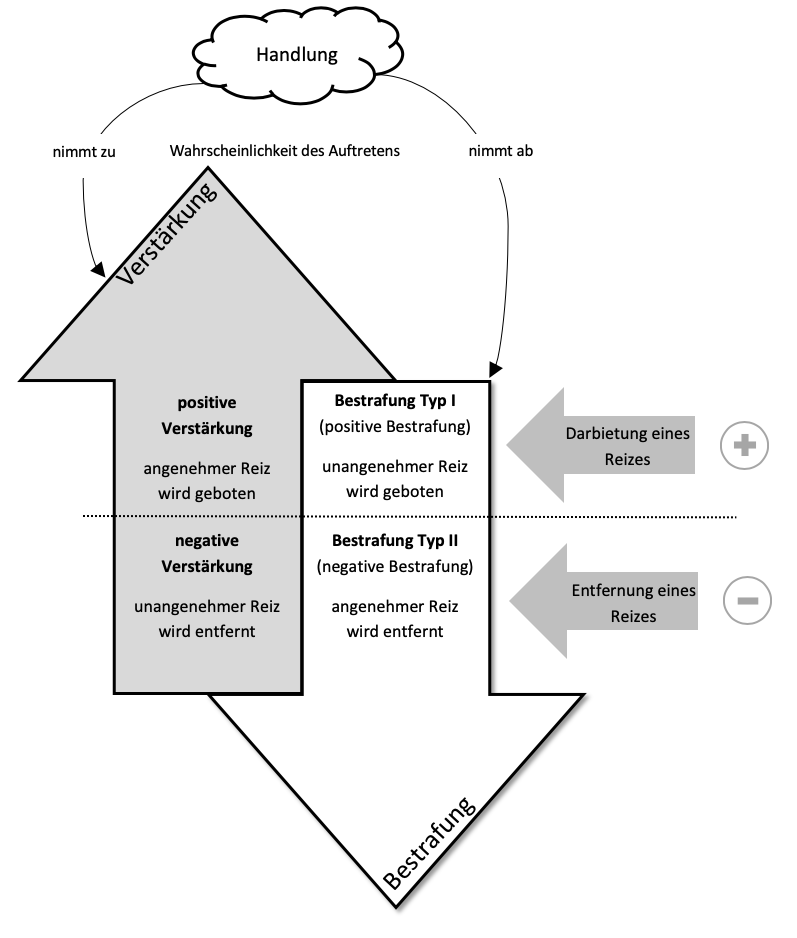
\includegraphics[width=10cm]{Kontingenzschema.png}
    \caption{Kontingenzschemata}
		\end{figure}
		\end{center}
		
		\begin{itemize}
			\item \textbf{Positive Verstärkung:} Erhöhung der Wahrscheinlichkeit des Auftritts einer Verhaltensweise, wenn die direkte Konsequenz des Verhaltens einer angenehmen Natur ist. 
			\item \textbf{Negative Verstärkung:} Erhöhung der Wahrscheinlichkeit des Auftritts einer Verhaltensweise, wenn das Verhalten eine unangenehme Konsequenz abwehrt.
			\item \textbf{Positive Bestrafung:} Senkung der Wahrscheinlichkeit des Auftritts einer Verhaltensweise, wenn das Verhalten eine unangenehme Konsequenz mit sich zieht.
			\item \textbf{Negative Bestrafung:} Senkung der Wahrscheinlichkeit des Auftritts einer Verhaltensweise, wenn das Verhalten eine angenehme Konsequenz verhindert. 
			\item \textbf{Extinktion:} Wenn eine Verhaltensweise, die zuvor durch Belohnung angelernt wurde auf ein Mal keine positiven Konsequenzen mehr mit sich zieht, wird diese immer seltener auftreten, bis die Verhaltensweise gar nicht mehr auftritt und somit „ausgestorben“ ist. 
		\end{itemize}
		
		
		\subsection{Arten von Verstärkern}
		
		Man unterscheidet grundsätzlich zwischen zwei verschiedenen Arten der Verstärker. Die primären und sekundären Verstärker. 
Ein primärer Verstärker zeichnet sich durch die Eigenschaft aus, dass eine Person mit diesen Reizen geboren wird. Essen, Trinken oder Schmerz sind zum Beispiel primäre Verstärker. \\
Sekundäre Verstärker sind Reize, die erlernt werden müssen. Am Anfang sind diese Verstärker neutrale Reize, die nach der Zeit mit Hilfe der primären Verstärker erlernt und gefestigt werden. Geld ist ein gutes Beispiel, da eine Person nach der Geburt nicht wissen kann, dass finanzieller Erfolg eine positive Änderung in Ihrem Leben widerspiegeln kann und erst gelernt werden muss. \\

		\subsection{Faktoren der Wirksamkeit der Verstärkung und Bestrafung}
		
		\begin{itemize}
			\item \textbf{Sättigung:} Die Wirksamkeit einer positiven Verstärkung nimmt ab, wenn die Person genug von dieser Belohnung hat. Die Person verliert Interesse.
			\item \textbf{Entzug:} Die Wirksamkeit einer positiven Verstärkung nimmt zu, wenn der Person die Stimulation dieser Belohnung entzogen wird. Wenn ein Verhalten mit Essen belohnt werden würde, hätte ein hungriges Tier eine größere Motivation als ein Tier, dass gerade gegessen hat. 
			\item \textbf{Unmittelbarkeit:} Eine unmittelbare Konsequenz hat einen signifikanteren Lernerfolg als eine verzögerte Konsequenz. 
			\item \textbf{Kontingenz:} Eine Konsequenz sollte immer regelmäßig nach einem Verhalten eintreten. Konsequenzen, die selten Erfolgen, werden langsamer erlernt, was bedeutet, dass das Verhalten seltener auftreten wird. 
			\item \textbf{Volumen:} Die Menge bzw. die Größe einer Belohnung erhöht bzw. senkt meistens die Wirkung der Verstärkung. 
		\end{itemize}
		
		%Quellen: 
		\subsection{Verstärkungspläne}
		
		Verstärkungspläne sind Methoden, die angewendet werden können, um Verhalten auf eine bestimmte Art zu konditionieren. \\ 
Verstärkungspläne treten sowohl in einer natürlichen Umgebung auf als auch in strukturierten Trainingssituationen auf. \\
Die durch B. F. Skinner definierten Verstärkungspläne sind: 

		\begin{itemize}
			\item Kontinuierliche Verstärkung
			\item Zeitpläne mit festem Verhältnis
			\item Zeitpläne mit festen Intervallen
			\item Zeitpläne mit variablem Verhältnis
			\item Zeitplänen mit variablen Intervallen
		\end{itemize}
		
		\subsection{Kontinuierliche Verstärkung}
		
		Bei jedem erwünschten Verhalten wird verstärkt, die Person lernt schneller aber verlernt dieses Verhalten wiederum auch schneller, wenn die kontinuierliche Verstärkung abnimmt oder beendet wird. \\
Eine kontinuierliche Verstärkung kann gut in der initialen Phase einer Konditionierung zur Verwendung kommen, um den Lernerfolg am Anfang stark zu steigern.\\
Um das Verlernen des Verhaltens vorzubeugen, müssen Verstärkungen nach bestimmten Zeitabständen neu durchgeführt werden. \\

		%Quellen: https://www.verywellmind.com/what-is-a-fixed-ratio-schedule-2795190 
		\subsection{Zeitpläne mit festem Verhältnis}
		
		Die Verstärkung tritt erst nach einer bestimmten Häufigkeit des Auftretens von erwünschten Verhaltensmustern auf.\\
Resultiert in häufigem und gleichmäßigem Auftreten von erwünschten Verhaltensmustern. Möglicherweise führt diese Methode zu einem kurzen Stopp der erwarteten Verhaltensweise, nachdem eine Belohnung gegeben wurde. \\
Kann sehr gut verwendet werden, um neue Verhaltensmuster zu lernen.\\

		%Quellen: https://www.verywellmind.com/what-is-a-fixed-interval-schedule-2795189
		\subsection{Zeitpläne mit festen Intervallen}
		
		Die Verstärkung wird erst nach einer definierten Zeit ausgegeben, wobei das Verhalten bei dieser Methode keine Rolle spielt. \\
Resultiert in einer signifikanten Pausierung der erwünschten Verhaltensmuster. Wenn es wieder Zeit für eine neue Verstärkung wird, treten die erwarteten Verhaltensmuster nach und nach immer häufiger auf. \\

		%Quellen: https://www.verywellmind.com/what-is-a-variable-ratio-schedule-2796012
		\subsection{Zeitpläne mit variablem Verhältnis}
		
		Die Verstärkung erfolgt, wenn ein erwünschtes Verhaltensmuster auftritt. Dabei kann auch definiert werden, dass die Verstärkung nach einer ungefähren Anzahl an Reaktionen erfolgt. Diese Eigenschaften machen diese Methode zu einem bestimmten Grad unvorhersehbar, und steigern die Lernkurve. \\
Zeigt erhöhte und gleichmäßige Wahrscheinlichkeit eines Verhaltens. Es tritt eine kurze Verhaltenspause nach der Verstärkung auf. \\

		%Quellen: https://www.verywellmind.com/variable-interval-schedule-2796011 
		\subsection{Zeitplänen mit variablen Intervallen}
		
		Verstärkung erfolgt nach einer zufälligen Zeit in einer vordefinierten Zeitspanne. \\
Diese Methode hat eine hohe Resistenz gegen Extinktion. Die Wahrscheinlichkeit einer erwünschten Reaktion ist moderat, aber konsistent und es gibt eine sehr kleine Verhaltenspause nach einer Belohnung. \\

		
		\subsection{Nichtkontingente Verstärkung}
		
		Nichtkontingente Verstärkung beschreibt die Abnahme von Verhaltensmustern unabhängig vom Verhalten der Person. Die Nichtkontingente Verstärkung kann verwendet werden, um die Wahrscheinlichkeit eines unerwünschten Verhaltens zu reduzieren, in dem man andere, Verhaltensmuster, die nicht erwünscht sein müssen, aber nicht, nicht erwünscht sind, belohnt und somit das unerwünschte Verhalten abtrainiert, ohne es selbst zu behandeln. \\

\chapter{Vorgehensweise}
\reiter
Es war ursprünglich geplant RUP\footcite{Lehrunterlagen-RUP} als Vorgehensmethode zu verwenden. 
\section{RUP}
RUP steht für Rational Unified Process und ist ein Prozessmodell, dass für die Software-Entwicklung konzipiert wurde und einen besonderen Schwerpunkt auf objektorientierte Entwicklung legt. Das Prozessmodell wurde von der Firma Rational entwickelt und besteht seit 1998 als RUP. Vorgängermodelle gibt es seit 1995. 
RUP berücksichtigt Best-Practices der Softwareentwicklung, also, Richtlinien, die aus Jahrelanger Erfahrung in der Industrie abgeleitet werden konnten. Pest-Practices müssen nicht zwingend befolgt werden, stellen aber für Entwickler einen guten Ansatz, der durch Erfahrene Herausgeber definiert worden ist, dar. 
RUP orientiert sich an Anwendungsfällen, die Anforderungen an das Gesamtsystem beschreiben. Anforderungen können als größere und ausführlicher definierte User-Stories gesehen werden.  
Der Projektablauf ist in vier Phasen aufgeteilt. Nach jeder Phase wird ein Meilenstein definiert, der inhaltlich klar beschrieben wurde.
Um die Projektziele erreichen zu können werden verschiedene Prozesse, einen Workflow, die, während jeder Phase als Querschnittsaufgabe, durchgeführt werden müssen, benötigt. Ein Workflow beschreibt welches Teammitglied welche Aufgabe zu welcher Zeit mit einem bestimmten Ergebnis durchzuführen hat.
In jeder Phase erfolgt die Entwicklung in kurzen Zyklen, die Iterationen genannt werden. Die Arbeit in einer Iteration ist auf die Erfüllung von Meilensteinen fokussiert. Am Ende einer Iteration sollte immer eine funktionsfähige Version des zu entwickelten Systems stehen. 
\subsection{Phasen}
\begin{itemize}
	\item \textbf{Inception-Phase:} Abgrenzung des Projektumfangs und genaue Beschreibung der wesentlichen Ziele. Es wird die Machbarkeit analysiert und der Aufwand festgestellt.
	\item \textbf{Elaboration:} Wichtigste Phase im Projekt. Hier sollte eine vollständige Analyse des Systems vorliegen. Es soll am Ende dieser Phase ein Prototyp vorliegen, der die wichtigsten Anforderungen beinhaltet.
	\item \textbf{Construction:} Hier finden die Entwicklung und das Testen der Applikation/Features statt.
	\item \textbf{Transition:} In dieser Phase soll ein Prototyp vorhanden sein der dem Auftraggeber übergeben werden kann. 
\end{itemize}
TODO: add aufwand und dauer pic
Diese Phasen werden genauer durch Phasenergebnisse sowie Meilenstein-Kriterien, die bei dem Übergang in die nächste Phase erfüllt werden müssen, beschrieben.
Die Anzahl der Iterationen in einer Phase wird durch den Schwierigkeitsgrad des Projekts bestimmt. 
\subsection{Iterationen}
Die kurzen Entwicklungszyklen\footcite{rup-workflows} der Iterationen in RUP ermöglichen ein frühzeitiges Feedback des Kunden, was hilft, dass späte Änderungen durch den Kunden vermieden werden können. 
\begin{center}
\begin{figure}[h]
	\centering
	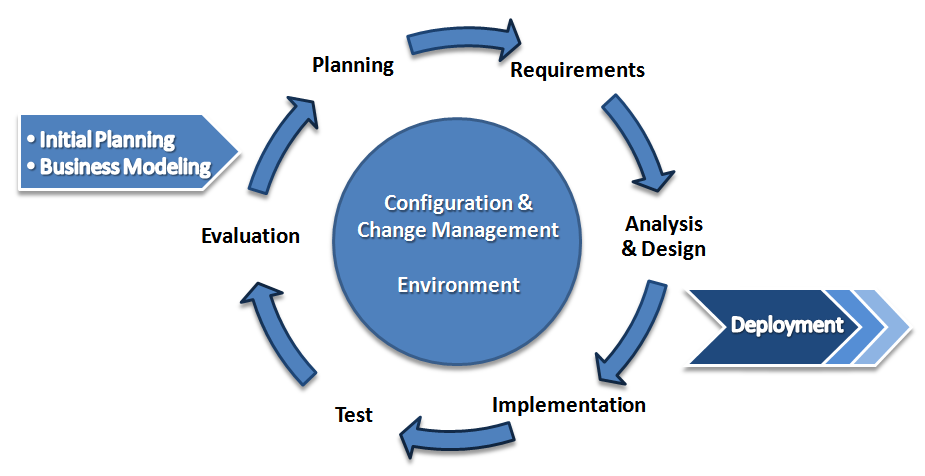
\includegraphics[width=\textwidth]{rup_iterationen.png}
	\caption{Iterationen in RUP}
\end{figure}
\end{center}
Die obenstehende Grafik zeigt alle Workflows einer Iteration. Die verschiedenen Workflows werden abhängig von der Phase der Iteration mit verschiedenen Intensitäten abgearbeitet. 
Es können mehrere Zyklen pro Iteration ablaufen.
Am Anfang jeder Iteration wird ein Iterationsplan erstellt, der die Aufgaben und Ziele einer jeden Iteration definiert. 
RUP trägt durch seine iterative Natur zur Vermeidung eines Late Design Breakages bei. Nicht iterative Modelle ermöglichen in einem frühen Stadium der Entwicklung keine Gesamtsicht auf das System. Mängel im System können erst spät erkannt werden. Somit müssen in vielen Komponenten der Software Änderungen vorgenommen werden, was einen hohen Aufwand darstellt und Verzögerungen im Deployment mit sich ziehen kann. 
Ein iterativer Entwicklungsansatz kann zwar nach jeder abgeschlossenen Phase auch Probleme offenlegen, diese sind aber auf Komponenten, die seit der zuletzt abgeschlossenen Phase erstellt wurden, begrenzt.
\subsection{Workflows}
\begin{itemize}
\item \textbf{Business Modelling:} Ein Business Model stellt die Geschäftsprozesse dar, für die Softwareentwickelt wird die diese umsetzt. Die Erstellung eines Business Models ist nicht zwingend notwendig.
\item \textbf{Requirements:} Es werden Anforderungen erstellt, die eine bessere Ansicht der zu entwickelnden Software ermöglichen soll. Diese Ansicht auf die Anforderungen des Projekts soll helfen, die Kommunikation zwischen Entwicklern und Stakeholdern, also Personen, die nicht im Entwicklerteam sind, wie zum Beispiel Kunden, zu vereinfachen.
\item \textbf{Analysis and Design:} Es wird der Systementwurf erstellt. Der Systementwurf ist ein Bauplan des Gesamtsystems, der die Entwicklung vereinfachen soll und allen Anforderungen der Funktionalität, Performance und Robustheit entspricht
\item \textbf{Implementation:} Es werden die Komponenten die im zuvor erarbeiteten Systemplan definiert wurden implementiert.
\item \textbf{Testing:} Die neu implementierten Komponenten werden getestet. Dieser Workflow findet im gesamten Projektverlauf statt.
\item \textbf{Deployment:} Stellt die Auslieferung an den Kunden dar. Es wird ein Release erstellt, gegebenenfalls beim Kunde installiert oder beim Umstieg des Kunden auf das neue vom alten System geholfen.
\end{itemize}
\subsection{Supporting Workflows}
\begin{itemize} 
	\item \textbf{Configuration and Change Management:} Kümmert sich um die Querschnittsaufgaben des Konfigurations- und Änderungsmanagements.
	\item \textbf{Project Management} 
	\item \textbf{Environment:} Anpassung des RUP an die sich ändernden Anforderungen im Projekt. Im Environment-Workflow werden auch alle Ressourcen, die zur Durchführung des Projekts benötigt werden zur Verfügung gestellt.
\end{itemize}
\section{SCRUM}
Im Rahmen der Anfangsarbeiten der Diplomarbeit wurde abteilungsintern die Verwendung der Projektmanagementsoftware Vivifyscrum vorgeschrieben. Durch diese Vorschrift konnte das Projekt nicht mit dem RUP-Prozessmodell entwickelt werden. 
Als Reaktion darauf wurde entschieden, dass SCRUM\footcite{Lehrunterlagen-SCRUM} als Prozessmodell verwendet werden soll.
\subsection{Rollen in Scrum}
Scrum hat grundsätzlich drei Rollen:
\begin{itemize} 
	\item \textbf{Product Owner:} dieser leitet das Projekt. Er vertritt das Team vor dem Auftraggeber, seine Aufgabe ist es die Erhebung, die Beschreibung und die Priorisierung der Anforderungen durchzuführen.
	\item \textbf{Scrum Master:} diese Person moderiert den Prozessablauf und versucht ihn voranzubringen. Er ist kein Mitglied des Entwicklungsteams.
	\item \textbf{Team} ist eine Gruppe von Entwicklern, die an dem Projekt arbeiten und für die Umsetzung der Arbeiten verantwortlich ist.
\end{itemize}
TODO grafik von Ablauf hinzufügen
\subsection{Product Backlog}
Bei Scrum gibt es den sogenannten Product Backlog, er beinhaltet alle Anforderungen, diese werden nach und nach in Sprints abgearbeitet.
\subsection{Sprint Planning Meeting}
Im Sprint Planning Meeting wird besprochen was im nächsten Sprint das voraussichtliche Ziel ist. Der Product Owner wählt die Arbeitspakete aus, die am höchsten priorisiert sind und in dem Sprint abzuarbeiten sind. Hier nehmen Product Owner, Scrum Master und das Team teil. 
\subsection{Sprint}
Ein Sprint ist die Phase, in der die Softwareentwicklung abgewickelt wird. Dieser dauert meist ein bis vier Wochen. 
\subsection{Daily Scrum}
Das Daily Scrum ist ein täglich in der Früh stattfindendes Meeting. Es werden Aufgaben vom Product Owner an das Team vergeben. Die Dauer eines solchen Meeting soll ungefähr 15 Minuten dauern.
\subsection{Sprint Review}
Das Sprint Review Meeting wird am Ende jedes Sprints abgehalten. Es wird ein lauffähiger Prototyp vorgestellt und es wird besprochen, wie der Sprint hinsichtlich abgearbeiteter Arbeitspakete verlaufen ist. Das Endergebnis soll zeigen ob alle Erwartungen des Kunden erfüllt wurden.
\subsection{Sprint Retrospektive}
Hier wird mit dem Scrum Master besprochen, wie der Arbeitsprozess bis zu diesem Zeitpunkt verlaufen ist. Das Ergebnis einer Sprint Retrospektive sind Maßnahmen, die den Entwicklern helfen sollen, zukünftige Sprints besser abschließen zu können.
\subsection{Fortschrittskontrolle}
Die nachfolgenden Methoden unterstützen die Planung, Durchführung und die Kontrolle des Arbeitsfortschrittes. 
\begin{itemize}
	\item	User Stories
	\item	Sprint Backlog
	\item	Burndown Chart
	\item	Timeboxing
	\item	Definition of Done
\end{itemize}
\subsection{User Stories}
Eine User Story gibt eine Anforderung vor. Der Kunde gibt unter Absprache mit dem Product Owner und dem Team alle User Stories am Anfang des Projekts an.
Anhand der User Stories kann der Fortschritt des Projekts gemessen werden.
Eine User Story ist eine zusammenfassende Einheit von ein oder mehreren Arbeitspaketen.
\subsection{Sprint Backlog}
Das Sprint Backlog stellt eine visuelle Darstellung dar, mit der der Fortschritt der Abarbeitung des Projekts dargestellt werden kann. Es werden auf einer Art Pinwand die User Stories, die im Sprint sind aufgelistet. Diese User Stories werden dann weiter in ihre Arbeitspakete aufgeteilt und können einen von drei Status, „offen“, „in Arbeit“ und „fertig“ haben.
\subsection{Burndown Chart}
Beim Burndown Chart wird der Verlauf des Projekts an den abgearbeiteten Tasks gemessen und bildlich dargestellt. In dem Diagramm beschreibt die x-Achse den Aufwand (in Personenstunden) bzw. die Anzahl von Tasks und die y-Achse die Arbeitstage des Sprints. 
Hierbei gibt es mehrere Linien, an denen der Fortschritt gemessen wird. Eine gibt die ideale Abarbeitung der Tasks an, eine den aktuellen Fortschritt in Tasks und eine den Fortschritt in Storypoints.
\subsection{Timeboxing}
Das Timeboxing zwingt ein Entwicklerteam Deadlines unbedingt einzuhalten. Sprints, die noch offene User Stories enthalten und zu Ende gegangen sind können nicht mit voller Funktionalität ausgeliefert werden. Die offenen User Stories müssen zurück in das Product Backlog geschoben und in den nächsten Sprint aufgenommen werden.
\subsection{Definition of Done}
Jeder User Story werden vom Scrum-Team klar definierten Kriterien zugewiesen, an denen Messbar sein soll, dass die User Story in Gänze und in akzeptierbarer Qualität abgeschlossen wurde.
\section{Scrum als Ablaufverfahren in der Entwicklung von EMS}
Am Anfang des Projekts wurden vom Team alle User Stories, die benötigt worden sind, um die gewünschten Funktionen von EMS realisieren zu können, definiert. Diese User-Stories wurden, soweit vom Umfang her möglich, in Tasks unterteilt. 
\begin{center}
\begin{figure}[H]
	\centering
	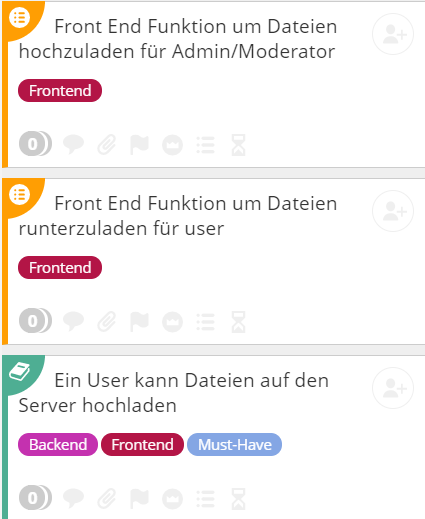
\includegraphics[width=6cm]{User-Story_Tasks.png}
	\caption{Beispiel einer User-Story mit Tasks}
\end{figure}
\end{center}
Nach der Definition wurden allen User-Stories vom Team gemeinsam eine geschätzte Abarbeitungsdauer und eine Priorität zugewiesen.  
User-Stories und die dazugehörigen Tasks wurden dann Sprints hinzugefügt, die eine Dauer von drei Wochen hatten. 
\begin{center}
\begin{figure}[H]
	\centering
	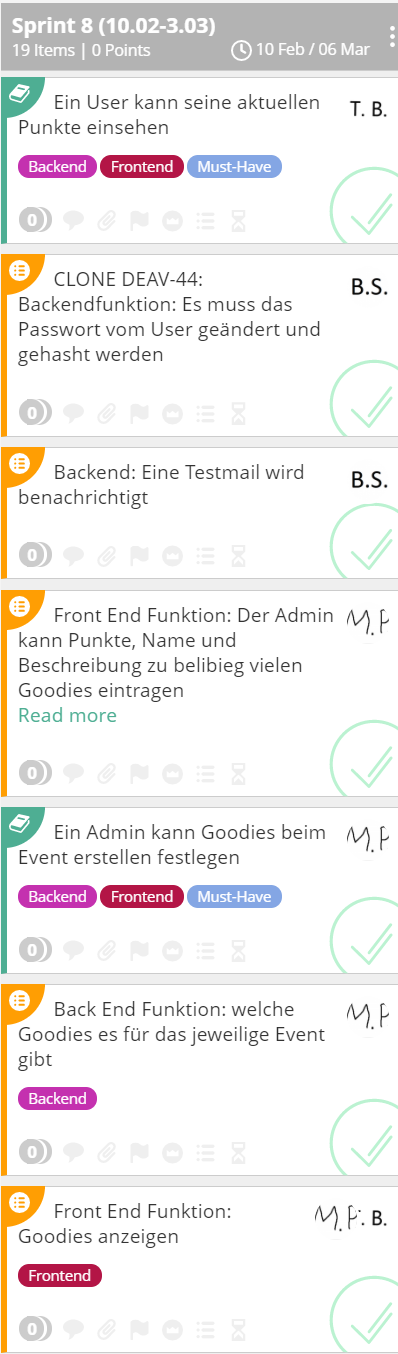
\includegraphics[width=6cm]{Sprint.png}
	\caption{Beispiel eines Sprints}
\end{figure}
\end{center}
Die Diplomarbeitsmitglieder konnten sich zum größten Teil ihre zu bearbeitenden User-Stories selbst aussuchen. Im Falle eines beendeten Sprints, der noch offene User-Stories aufwies, wurden die betroffenen User-Stories wieder zurück in das Product Backlog verschoben und bei Beginn des nächsten Sprints diesem wieder hinzugefügt.
\begin{center}
\begin{figure}[H]
	\centering
	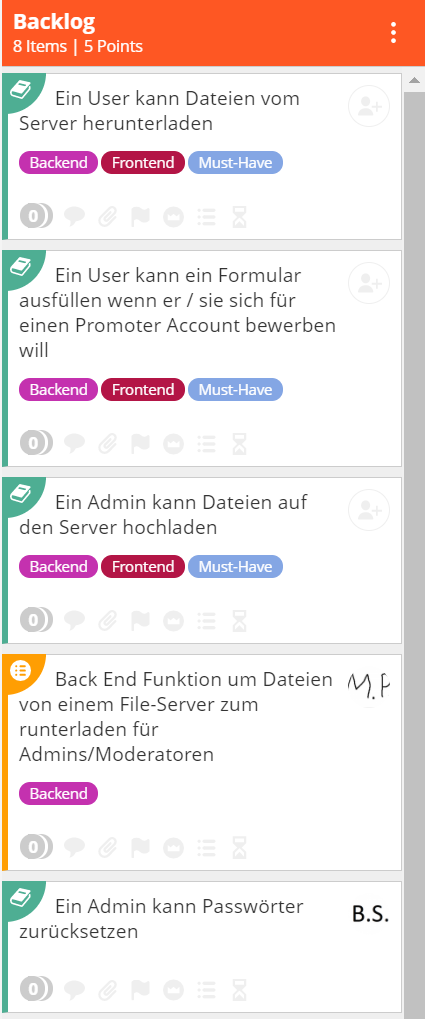
\includegraphics[width=6cm]{product_backlog.png}
	\caption{Product Backlog}
\end{figure}
\end{center}

Bruder gar kein Bock mehr auf sowas
%%%----------------------------------------------------------
%%%Anhang
%%%----------------------------------------------------------
%\appendix

%%Hier kommen die Includes für den Anhang

%%%----------------------------------------------------------
%Ausgabe der automatischen Zusatzdaten: Glossar, Index, Literaturverzeichnis
%\clearpage
%\printglossaries

\clearpage
\chapter*{Index}
\addcontentsline{toc}{chapter}{Index}
\printindex[allgemein]
\printindex
\printindex[name]
\printindex[title]

%Literaturverzeichnis
\clearpage
\addcontentsline{toc}{chapter}{\bibname}
\printbibliography
\clearpage
\chapter*{Messbox zur Druckkontrolle}



\begin{center}
{\Large --- Druckgröße kontrollieren! ---}

\bigskip

\Messbox{100}{50} % Angabe der Breite/Hoehe in mm

\bigskip

{\Large --- Diese Seite nach dem Druck entfernen! ---}

\end{center}



%%%----------------------------------------------------------
\end{document}